\documentclass{include/thesisclass}
% Main File - Based on thesisclass.cls
% Comments are mostly in English
% ------------------------------------------------------------------------------
% Further files in folder:
%  - include/cmds.tex (for macros and additional commands)
%  - include/kitlogo.pdf (for titlepage)
%  - lit.bib (bibtex bibliography database)
%  - include/titlepage.tex (for layout of titelpage)
% ------------------------------------------------------------------------------
% Useful Supplied Packages:
% amsmath, amssymb, mathtools, bbm, upgreek, nicefrac,
% siunitx, varioref, booktabs, graphicx, tikz, multicol



%% -------------------------
%% |    Thesis Settings    |
%% -------------------------
% english or ngerman (new german für neue deutsche Rechtschreibung statt german)
\SelectLanguage{ngerman}
% details on this thesis
\newcommand{\thesisauthor}{Max Erhart}
\newcommand{\thesistopic}{Machbarkeitsstudie für den Ionisationskanal eines Prototyp-Detektors zur Suche nach Leichter Dunkler Materie}
\newcommand{\thesisentopic}{}
\newcommand{\thesislongtopic}{}
\newcommand{\thesisinstitute}{Institut für Experimentelle Kernphysik}
\newcommand{\thesisreviewerone}{Prof. Dr. G. Drexlin}
\newcommand{\thesisreviewertwo}{Dr. K. Eitel}
\newcommand{\thesisadvisorone}{Dr. B. Siebenborn} % to use: enter names and uncomment in titlepg
\newcommand{\thesisadvisortwo}{}
\newcommand{\thesistimestart}{} % on titlepage
\newcommand{\thesistimeend}{} % on titlepage
\newcommand{\thesistimehandin}{} % on second page 'preamble'
\newcommand{\thesispagehead}{\thesisentopic} % page heading

\usepackage[nohyperlinks, printonlyused]{acronym}


%% ---------------------
%% |    PDF - Setup    |
%% ---------------------
% This information will appear embed into the PDF file as meta data, but will 
% not be printed anywhere
\hypersetup
{
    pdfauthor={\thesisauthor},
    pdftitle={Bachelorarbeit: \thesistopic},
    pdfsubject={\thesislongtopic},
    pdfkeywords={kit,physik,bachelor,thesis,\thesisauthor}
}



\DeclareSIUnit\year{y}

%% --------------------------------------
%% |    Settings for Word Separation    |
%% --------------------------------------
% Help for separation:
% In German package the following hints are additionally available:
% "- = Additional separation
% "| = Suppress ligation and possible separation (e.g. Schaf"|fell)
% "~ = Hyphenation without separation (e.g. bergauf und "~ab)
% "= = Hyphenation with separation before and after
% "" = Separation without a hyphenation (e.g. und/""oder)

% Describe separation hints here:
\hyphenation
{
    über-nom-me-nen an-ge-ge-be-nen
    %Pro-to-koll-in-stan-zen
    %Ma-na-ge-ment  Netz-werk-ele-men-ten
    %Netz-werk Netz-werk-re-ser-vie-rung
    %Netz-werk-adap-ter Fein-ju-stier-ung
    %Da-ten-strom-spe-zi-fi-ka-tion Pa-ket-rumpf
    %Kon-troll-in-stanz
}


\bibliography{bibly}
\DefineBibliographyStrings{ngerman}{andothers={et\addabbrvspace al\adddot}}                                    


%% -----------------------
%% |    Main Document    |
%% -----------------------
\begin{document}


    % Titlepage and ToC
    \FrontMatter

    % coordinates for background border
\newcommand{\diameter}{20}
\newcommand{\xone}{-15}
\newcommand{\xtwo}{160}
\newcommand{\yone}{15}
\newcommand{\ytwo}{-253}




\begin{titlepage}
    % background border
    \begin{tikzpicture}[overlay]
    \draw[color=gray]
            (\xone mm, \yone mm)
      -- (\xtwo mm, \yone mm)
    arc (90:0:\diameter pt)
      -- (\xtwo mm + \diameter pt , \ytwo mm)
        -- (\xone mm + \diameter pt , \ytwo mm)
    arc (270:180:\diameter pt)
        -- (\xone mm, \yone mm);
    \end{tikzpicture}



    % KIT image and sign for faculty of physics
    \begin{textblock}{10}[0,0](4.5,2.5)
        
\includegraphics[width=.25\textwidth]{include/kitlogo.pdf}
    \end{textblock}
    \changefont{phv}{m}{n}    % helvetica
    \begin{textblock}{10}[0,0](5.5,2.2)
        \begin{flushright}
            \Large FAKULTÄT FÜR PHYSIK\\\thesisinstitute
        \end{flushright}
    \end{textblock}



    % horizontal line
    \begin{textblock}{10}[0,0](4.2,3.1)
        \begin{tikzpicture}[overlay]
        \draw[color=gray]
                (\xone mm + 5 mm, -12 mm)
          -- (\xtwo mm + \diameter pt - 5 mm, -12 mm);
        \end{tikzpicture}
    \end{textblock}



    % begin of text part
    \changefont{phv}{m}{n}    % helvetica
    \centering



    % thesis topic (en and ge)
    \vspace*{3cm}
    \Huge\thesistopic\\
    %\huge(\thesisentopic)\\



    % author name and institute
    \vspace*{2cm}
    \Large Bachelorarbeit\\von\\
    \vspace*{1cm}
    \huge\thesisauthor\\
    \vspace*{1cm}
    \Large am \thesisinstitute



    % possible frontimage - thanks to JabberWok
    % for publishing the img under GNU Document License
    %\vspace*{1.5cm}
    %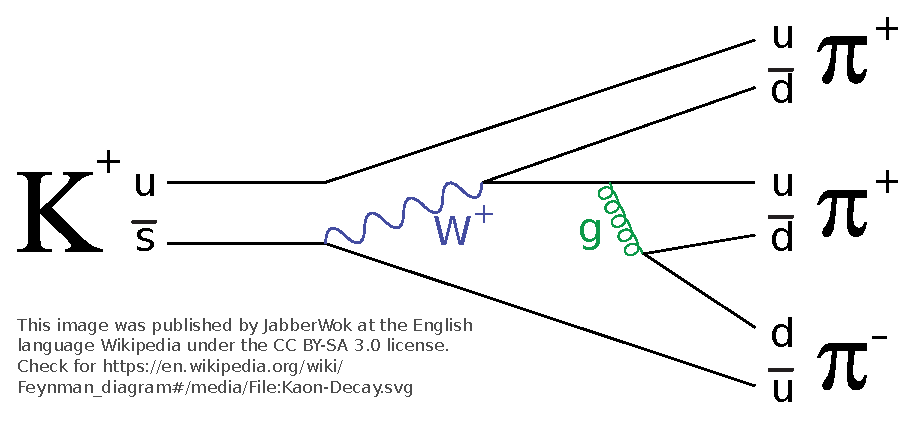
\includegraphics[scale=0.7]{./include/frontimage.eps}\\



    % examiners (Referenten)
    \vspace*{1.5cm}
    \Large
    \begin{center}
        \begin{tabular}[ht]{l c l}
        \iflanguage{english}{Reviewer}{Referent}: 
            & \hfill & \thesisreviewerone\\
        \iflanguage{english}{Second Reviewer}{Koreferent}: 
            & \hfill & \thesisreviewertwo\\
        % uncomment if you want to provide info on your advisors
        \iflanguage{english}{Advisor}{Betreuender Mitarbeiter}: 
            & \hfill & \thesisadvisorone\\
        %\iflanguage{english}{Second Advisor}{Zweiter betreuender Mitarbeiter}: 
        %    & \hfill & \thesisadvisortwo\\
        \end{tabular}
    \end{center}



    % working time
    \vspace{1cm}
    \begin{center}
        \large{{Bearbeitungszeit}: \thesistimestart \hspace*{0.25cm} -- %
                                   \hspace*{0.25cm} \thesistimeend}
    \end{center}



    % lowest text blocks concerning the KIT
    \begin{textblock}{10}[0,0](3,16.8)
        \tiny{KIT -- Universität des Landes Baden-Württemberg und nationales %
              Forschungszentrum in der Helmholtz-Gemeinschaft}
    \end{textblock}
    \begin{textblock}{10}[0,0](10,16.75)
        \large{\textbf{www.kit.edu}}
    \end{textblock}
\end{titlepage}

    \chapter*{Erklärung zur Selbstständigkeit}
Ich versichere, dass ich diese Arbeit selbstständig verfasst habe und keine %
anderen als die angegebenen Quellen und Hilfsmittel benutzt habe, die %
wörtlich oder inhaltlich übernommenen Stellen als solche kenntlich gemacht und %
die Satzung des KIT zur Sicherung guter wissenschaftlicher Praxis in der %
gültigen Fassung vom 17.05.2010 beachtet habe.\\

\vspace{1cm}

\renewcommand{\arraystretch}{0} % for spacing in the tabular environment

\begin{flushright}
	\begin{tabular}{rr}
		Karlsruhe, den \thesistimehandin, & \hspace*{5cm}\\[0mm]
		\cline{2-2}\vspace{1mm}\\[2mm]    % the last line has height 2mm due
		& \thesisauthor       % to \arraystretch=0
	\end{tabular}
\end{flushright}

\vfill

\begin{flushright}
	Als Ansichtsexemplar genehmigt von\\
	\vspace{1cm}
	\begin{tabular}{rr}
		Karlsruhe, den \thesistimehandin, & \hspace*{5cm}\\[0mm]
		\cline{2-2}\vspace{1mm}\\[2mm]    % the last line has height 2mm due
		& \thesisreviewerone  % to \arraystretch=0
	\end{tabular}
\end{flushright}

\renewcommand{\arraystretch}{1}

\cleardoublepage


    \begingroup \let\clearpage\relax    % in order to avoid listoffigures and
    \tableofcontents                    % listoftables on new pages
    \endgroup
    \cleardoublepage



    % Contents
    \MainMatter

    \addchap{Einleitung}
    Der Großteil der Masse im Universum besteht aus nicht sichtbarer \ac{DM} deren Existenz durch kosmologische Beobachtungen begründet ist.
Die Zusammensetzung von \acs{DM} ist bis heute unklar. 
Das Untersuchen von \acs{DM} gibt uns nicht nur Aufschluss über ihre Eigenschaften wie Zusammensetzung, Wechselwirkung und Herkunft, sondern ermöglicht gleichzeitig Erkenntnisgewinn über die Entstehung des Universums.
Prinzipiell liegt ein Fokus jüngerer Experimente auf dem Nachweis einer Streuung von \ac{DM} mit sichtbarer Materie. 

Viel Aufwand wurde in die Detektion von \acp{WIMP} als Kandidaten für DM im Massenbereich von wenigen GeV bis TeV gesteckt.
Auf Direktem Wege wird anhand \ac{DM}-Nukleon Streuung nach \acp{WIMP} gesucht.
Zu diesen Experimenten zählen zum Beispiel \acs{XENON}\cite{Aprile2017} und \acs{LUX}\cite{DaSilva2017} welche flüssige Edelgase als Detektormaterial verwenden.
Alternativ werden hochreine Halbleiterkristalle bei kryogenen Temperaturen verwendet.
Experimente wie \acs{EDELWEISS}\cite{EDWIII} oder \acs{SuperCDMS}\cite{Agnese2018} verwenden Germanium Kristalle in einem elektrischen Feld.
Um hohe Sensitivität zu erreichen werden die Detektoren auf Temperaturen von wenigen Kelvin gekühlt.
Die bei einer Wechselwirkung im Germaniumkristall deponierte Energie in Form von Ionisation, Szintilationslicht oder Wärme (Phononen) ist messbar und gibt Aufschluss über die wechselwirkenden Teilchen. 
Die Informationen über das Ereignis werden bei EDELWEISS durch das Auslesen des Ionisationssignals sowie des Phononsignals gewonnen.
Die Verwendung beider Kanäle ermöglicht zusätzlich zur Energiebestimmung zwischen Kern- und Elektron Streuung zu diskriminieren.
Auf diese Art können große Teile des Parameterbereichs von \acp{WIMP} abgedeckt werden.
Bisher konnte allerdings kein eindeutiges \ac{WIMP} Signal festgestellt werden.
Neben \acp{WIMP} ist \ac{LDM} mit Massen im sub-GeV Bereich eine vielversprechende Möglichkeit.
Das DELight Experiment hat das Ziel mittels \ac{DM}-Elektron Streuung die Sensitivität im Bereich \ac{LDM} um mehrere Größenordnungen zu verbessern.
Dazu soll mittels Luke-Verstärkung (siehe Abschnitt \ref{sec:LukeAmp}) eine Energieauflösung des Ionisationssignals im $\SI{}{\electronvolt}$ Bereich erreicht werden.

Der Aufbau sieht für das Einbringen des elektrischen Feldes vakuumseparierte Elektroden vor.
Dies verbessert einerseits die Qualität des Wärmekanals erhöht aber andererseits die Anforderungen für die Messung im Ionisationskanal.
Die Aufgabe in dieser Arbeit ist es zu untersuchen, ob es möglich ist an den vakuumseparierten Elektroden ein Signal im Ionisationskanal zu messen.
Dazu ist es notwendig die Verstärkerelektronik des Ionisationskanal zu entwickeln und deren Auflösung zu untersuchen.
Ziel ist es die Messanordnung in zukünftigen Arbeiten anzuwenden, um die Linearität des Neganov-Luke-Effekts in einem großen Spannungsbereich zu prüfen.



    
    \chapter{Dunkle Materie}
    \section{Evidenzen für Dunkle Materie}
    Erste Beobachtungen der Effekte von Dunkler Materie wurden von Fritz Zwickey im Jahr 1933 gemacht.
Unter Verwendung des Virialsatzes der Thermodynamik berechnete er die Rotantionsgeschwindigkeit von Galaxien im Coma Cluster basierend auf der leuchtenden Materie.
Diese verglich er mit den über die Rotverschiebung bestimmten Rotationsgeschwindigkeiten und fand, dass die Masse ungefähr um eine $400$ faches kleiner ist als erwartet.\cite{Zwicky1933}
Um die Diskrepanz zu erklären postulierte er weitere nicht leuchtende Materie, Dunkle Materie.
Bis Heute wurden zahlreiche weitere Beobachtungen der Effekte von DM gemacht.
Erwartet wird, dass die gesamte Materie zu $\SI{84}{\percent}$\cite{Adam2016} aus DM besteht.
Im Folgenden werden die prominentesten dieser Beobachtungen vorgestellt.

\begin{figure}[!b]
\begin{center}
\includegraphics[width=0.8\textwidth]{./fig/Rubin80.pdf}
\end{center}
\caption{Rotationsgeschwindigkeit in Abhängigkeit des Radius zum Zentrum für 21 Sc Galaxien.\cite{Rubin80}}
\label{fig:Rubin21Sc}
\end{figure}

\subsection*{Rotationskurven von Galaxien}
Für die Rotationsgeschwindigkeit von Galaxien erwarten wir anhand der newtonschen Mechanik
\begin{equation}
v(R) = \sqrt{\frac{GM(R)}{R}}
\label{eq:Keppler}
\end{equation}
hier ist $G$ die Gravitationskonstante, $R$ der Abstand zum Zentrum der Rotation und $M(R)$ die gesamte Massen innerhalb einer Kugel des Radius $R$ um das Zentrum.  
Ab einem gewissen Abstand ist der Großteil der sichtbaren Masse von dieser Kugel eingeschlossen.
Ab dann bleibt $M(R)$ ungefähr konstant und die Rotationsgeschwindigkeit nimmt mit $1/\sqrt{R}$ ab.
Dieses verhalten wurde mittels Rotverschiebung von Vera Rubin in den 70er Jahren anhand von Spiralgalaxien untersucht.
Mit dem Ergebnis, dass die Rotationskurven aller von ihr untersuchten Galaxien konstant bleiben oder sogar ansteigen weit jenseits ihrer größten Leuchtkraft, siehe Abbildung \ref{fig:Rubin21Sc}.
Dies suggeriert eine nicht leuchtende, linear mit dem Radius ansteigende Massenverteilung.\cite{Rubin80}
Jüngste Beobachtungen zeigen, dass auch Galaxie mit fast keiner DM auftreten können\cite{VanDokkum2018}.
Dunkle Materie und Baryonische Materie sind daher nicht immer aneinander gekoppelt wie es für Theorien wie MOND\cite{1983ApJ...270..365M} (\textit{Modified Newtonian dynamics}) und emergent gravity paradigm\cite{Verlinde2016} notwendig ist in denen die Effekte Dunkle Materie eine Konsequenz Baryonischer Materie sind.

\begin{figure}[!b]
\begin{center}
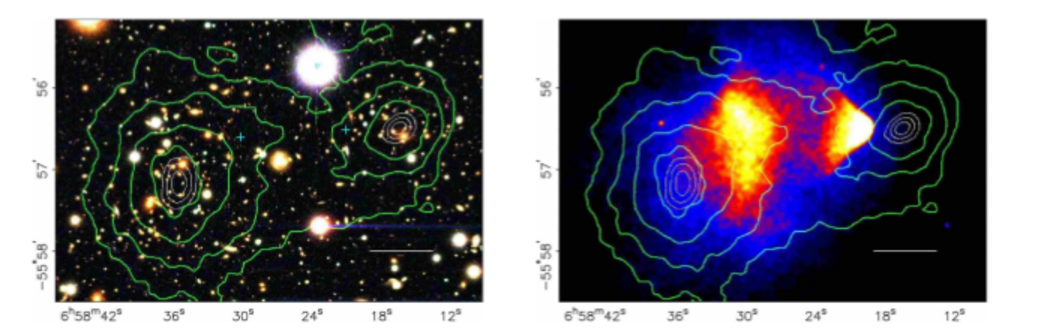
\includegraphics[width=\textwidth]{./fig/Bullet.pdf}
\end{center}
\caption{Links:Aufnahme des Bullet Cluster vom Magellan Teleskop.
Rechts: Röntgenaufnahme des Bullet Cluster vom Chandra Teleskop.
Die Konturen zeigen die durch den schwachen Gravitationslinseneffekt erwartete Massenverteilung.\cite{Clowe2006}}
\label{fig:BulletC}
\end{figure}

\subsection*{Evidenz aus Gravitationslinseneffekten}
Als Gravitationslinseneffekt wird die Ablenkung von Licht durch die Raumkrümmung massereicher Objekte bezeichnet und führt dazu, dass Objekte vergrößert, verzerrt oder heller erscheinen\cite{Massey2010}.
Mittels des schwachen Gravitationslinseneffekt wurde außergewöhnliche Erkenntnisse über die Massenverteilung im Bullet Cluster gewonnen.
Das Bullet Cluster besteht aus zwei kollidierten Clustern.
Bei der Kollision sind die Galaxien der Cluster fast ungehindert passiert.
Der Großteil der Clustermassen in Form von interstellarem Gas befindet sich allerdings noch im Zentrum der Kollision und erzeugt Röntegnstrahlung auf Grund Elektromagnetischer Wechselwirkungen, in Abb. \ref{fig:BulletC} links dargestellt.
Die durch den schwachen Gravitationslinseneffekt bestimmte Massenverteilung zeigt allerdings weitere um die ursprünglichen Cluster verteilte Materie welche bei der Kollision kaum wechselwirkte.
Aus der Position des warmen Gas und der Position der Dunklen Materie kann die Größe der Selbstwechselwirkung von Dunkler Materie eingeschränkt werden.\cite{Markevitch2003}

    \section{Teilchenkandidaten für Dunkle Materie}
    Aus den beobachteten Effekten Dunkler Materie lassen sich bereits Eigenschaften ableiten, welche von Teilchenkandidaten erfüllt sein müssen.
Dunkle Materie interagiert nur sehr schwach, ist stabil auf der kosmologischen Zeitskala und ist zum Großteil kalt (nicht relativistisch).
Die Liste möglicher Kandidaten ist zahlreich.
Von besonderem Interesse sind diejenigen, die zusätzlich aus anderen Teilgebieten der Physik motiviert sind.

\subsection*{Axion}
\acs{CP}-Verletzung sollte in der starken Wechselwirkung möglich sein, konnte bisher allerdings nicht beobachtet werden.
Die Abwesenheit von CP-Verletzung in der starken Wechselwirkung ist als starkes CP-Problem bekannt.
Durch das Hinzufügen einer $U(1)$ \ac{PQ} Symmetrie kann dieses gelöst werden.\cite{Peccey1977}
Das Axion ist das Nambu-Goldstone Boson der spontanen Brechung dieser Symmetrie.
Aufgrund stellarer Entwicklung wird erwartet, dass die Masse des Axions kleiner als $\SI{e-2}{\electronvolt}$\cite{Raffelt1999} ist.
Nicht thermische Axionen könnten trotzdem ein Kandidat für kalte DM sein.\cite{Drees2012}
Eine Auswahl verschiedener Ausschlussbereiche für die Axionmasse und die Kopplung an zwei Photonen ist in Abb. \ref{fig:AxionExclusion} gegeben.

\begin{figure}[!b]
\begin{center}
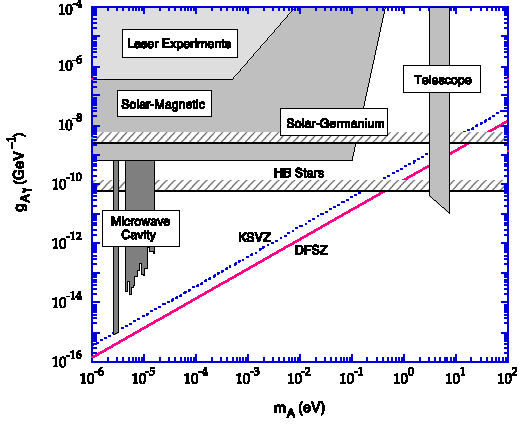
\includegraphics[width=0.8\textwidth]{./fig/AxionExclusion.pdf}
\end{center}
\vspace{-0.5cm}
\caption{Ausschlussbereiche der Axionmasse und Kopplung an zwei Photonen.
Auf der vertikalen Axe ist die effektive Kopplung des Axions an zwei Photonen aufgetragen und auf der horizontalen die Masse.
KSVZ und DSVZ sind zwei Klassen von Axion Modellen.
DM Axionen werden zwischen diesen Modellen im Massenbereich von $\SI{1}{\mu\electronvolt}\--\SI{100}{\mu\electronvolt}$ erwartet.\cite{Rosenberg2010}}
\label{fig:AxionExclusion}
\end{figure}

\subsection*{WIMPs}
Als WIMP (weakly interacting massive particles) wird eine Gruppe von Teilchen bezeichnet, welche eine Masse im Bereich von $\SI{10}{\giga\electronvolt}\--\SI{1}{\tera\electronvolt}$ haben und Wirkungsquerschnitte in der Größenordnung schwacher Wechselwirkungen\cite{Drees2012}.
WIMPs entstanden im frühen Universum im thermischen und chemischen Gleichgewicht mit Teilchen des \ac{SM}. 
Beim Abkühlen des Universums fällt die Anzahl der WIMPs ab einer Temperatur kleiner der WIMP Masse, aufgrund des Boltzmann-Faktors, exponentiell ab.
Da sich das Universum allerdings gleichzeitig ausdehnt kommt es ab dem Punkt an dem die Paarvernichtungsrate kleiner als die Expansionsrate des Universums ist, zum Freeze-out und die Teilchendichte bleibt nahezu konstant.
Es bleibt eine so genannte relic density übrig.
Liegt der Wirkungsquerschnitt für WIMPs in der Größenordnung schwacher Wechselwirkungen, ergibt sich für die relic density die aus kosmologischen Beobachtungen erwartete DM Dichte.
Dies wird als WIMP miracle bezeichnet.
Eigentlich motiviert als Lösung des gauge hirachy problem tauchen in der \ac{SUSY} mögliche WIMP Kandidaten auf.
SUSY ist eine Erweiterung des SM in dem eine Symmetrie zwischen Fermionen und Bosonen eingeführt wird.
Dies fordert weitere Teilchen welche sich im Spin um $1/2$ zu ihrem SM Partner unterscheiden.
Das leichteste supersymmetrische Teilchen ist aufgrund der neuen Erhaltungsgröße R-Parität stabil und daher ein möglicher WIMP Kandidat.
Dieses könnte das Neutralino sein.\cite{Feng2010}

%\subsection*{Sterile Neutrinos}


    \section{Direkter Nachweis Dunkler Materie}
    Der Nachweis DM durch Streuung an einem SM Teilchen wird als direkter Nachweis bezeichnet.
Dabei wird im Experiment die bei der Streuung deponierte Energie in Form von Ionisation, Szintillationslicht oder Phononen bestimmt.
Die Rate solcher Ereignisse ist entscheidend von der Dichte, relativen Geschwindigkeit zwischen Erde und DM-Halo, Masse der DM Teilchen und Wirkungsquerschnitt der Wechselwirkung abhängig.
Aufgrund des kleinen Wirkungsquerschnitt ist genaue Kenntnis und Minimierung des Untergrunds notwendig.
Daher befinden sich Experimente dieser Art in Laboren tief unter der Erde.
Aufgrund natürlicher Radioaktivität wird der Untergrund zusätzlich durch aktive und passive Schilde sowie hochreines Detektormaterial verringert.

Im Wesentlichen gibt es zwei Arten von Detektor Typen kryogene Halbleiterdetektoren und Edelgasdetektoren mit flüssigem Edelgas.
Flüssig Edelgasdetektoren verwenden Photomultiplier um das Scintillationslicht welches bei Wechselwirkungen entsteht zu detektieren.
Zusätzlich driften die Ladungsträger des Ionisationssignal im extern angelegten Feld und erzeugen dabei weiteres Szintillationslicht.
Dadurch kann zwischen Nukleon und Elektron Streuung unterschieden werden.
Der Detektor fungiert dadurch als Time Projection Chamber.
Aktuell wird als Detektormaterial flüssiges Xenon oder flüssiges Argon verwendet.
Experimente dieser Art sind XENON\cite{Aprile2017} und LUX\cite{DaSilva2017}.
Kryogene Halbleiterdetektoren sind hochreine Kristalle welche im $\SI{}{\milli\kelvin}$ Bereich angewendet werden.
Über Sensoren an der Oberfläche wird anhand des Wärme- und Ionisationssignal die deponierte Energie bestimmt.
Prominente Beispiele für Experimente dieser Art sind EDELWEISS\cite{EDWIII} und SuperCDMS\cite{Agnese2018}.
    %\section{Methoden zum Nachweis von Dunkler Materie}
	%Aus dem Einfluss DM aufgrund von gravitativen Effekten lässt sich nur ein unvollständiges Bild ihrer Zusammensetzung ableiten.
Daher wird auf viele verschiedene Arten versucht Aufschluss über ihre Eigenschaften zu gewinnen.
Die dabei verwendeten Methoden können in drei Klassen entsprechend 

\subsection*{Indirekter Nachweis}

Messungen von Teilchen des Standardmodells, welche bei der Annihilation oder dem Zerfall von Dunkler Materie entstehen, wird als Indirekter Nachweis bezeichnet. 
Die Rate solcher Ereignisse ist in Gebieten hoher DM Dichte am größten.
Eine große Schwierigkeit bei der indirekten Suche sind die zahlreichen unterschiedlichen Quellen von Teilchen, welche eine ähnliche Signatur aufweisen.

Experimente wie H.E.S.S. oder VERITAS nutzen Cherenkov Teleskope um in Zentren von Galaxien nach Dunkler Materie zu suchen.
Das Weltraumteleskop PAMELA berichtete 2009 von einem 9 bis 275$\si{\giga\electronvolt}$ Positron zu Elektron Überschuss.
Das AMS-02 Experiment auf der \textit{International Space Station} konnte diese Ergebnisse bestätigen.
Um aus diesen Ergebnisse eindeutig auf die Annihilation von Dunkler Materie zu schließen ist eine genauso großer Überschuss von Protonen zu Antiprotonen notwendig.
Dieser konnte bisher nicht beobachtet werden.\cite{PAMELA}
    
	\chapter{Suche nach LDM mit DELight}
	\begin{figure}[!b]
\begin{center}
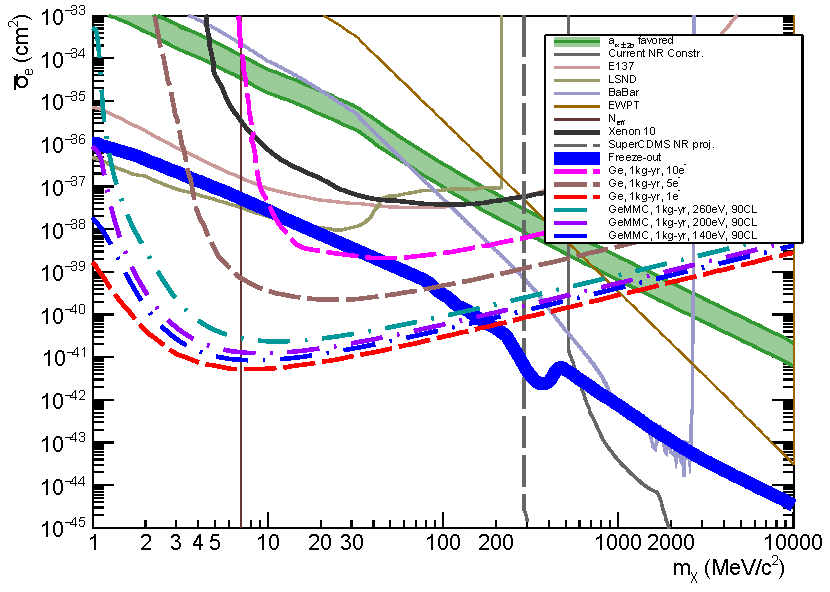
\includegraphics[scale=1]{./fig/DMElektronStreuung.pdf}
\vspace{-0.5cm}
\caption{Sensitivitätskurve für einen DM-Formfaktor FDM = 1 in Kombination
mit Ausschlusskurven anderer Experimente für den DELight Detektor. Die dicke blaue
Linie stellt den durch Freeze-out favorisierten Parameterbereich da.\cite{Lukwata2017}}
\label{fig:DMES}
\end{center}
\end{figure}

Trotz großem experimentellem Aufwand konnte bisher kein eindeutiges WIMP Signal beobachtet werden.
Der theoretisch Motivierte Parameterbereich LDM (light dark matter) von $\SI{}{\mega\electronvolt}\--\SI{}{\giga\electronvolt}$ ist allerdings noch weitgehend unerforscht.
Ziel des DELight Experiment ist es die Sensitivität im Massenbereich von $\SI{1}{\mega\electronvolt}\--\SI{10}{\mega\electronvolt}$ um mehrere Größenordnungen zu verbessern.
Um dieses zu erreichen wird das Ionisationssignal weniger Elektronen einer DM-Elektron Streuung betrachtet\cite{Essig2016}.
Als Target wird Germanium verwendet welches sich aufgrund seiner geringen effektiven Bandlücke von $\SI{3}{\electronvolt}$ besonders gut eignet.\cite{Essig2012}
Neben Neutrinos ist der Untergrund weitgehend unbekannt.
Eine wichtige Methode um Signal vom Untergrund zu unterscheiden ist die jährliche Modulation des Flusses an DM aufgrund der relativen Geschwindigkeit zwischen dem DM halo und der Erde\cite{Drukier1986}.
Allerdings gibt es für Signale wie sie von LDM erwartet werden kaum Untergrund.
In Abb. \ref{fig:DMES} ist die erwartete Sensitivität des GeMMC Detektors für eine Untergrundfreie Exposition von $\SI[inter-unit-product = \cdot]{1}{\kilogram\year}$ dargestellt.


	\section{Konzept des DELight Experiments}
	\begin{figure}[!b]
\begin{center}
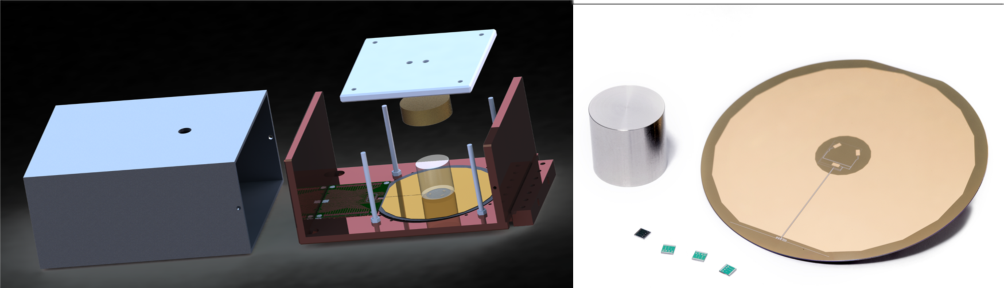
\includegraphics[width=\textwidth]{./fig/Antrag-DELight-extract.pdf}
\vspace{-0.5cm}
\caption{Links: Schema des DELight Aufbaus mit dem zylinderförmigen Detektor auf den drei MMCs und der entsprechenden Halterung inklusive der Vakuum Kupferelektrode. Rechts: Germaniumkristall, dreieckige MMC Struktur und SQUID-holding Chips.}
\label{fig:DELightAufbau}
\end{center}
\end{figure}
\todo{CITE SCHEMATIC \ref{fig:DELightAufbau}}
Bei einer DM-Elektron Streuung entsteht eine bestimmte Anzahl Elektron-Loch-Paare im Germanium Target.
Diese soll bestimmt werden, da sie Aufschluss über die deponierte Energie gibt.
Dazu wird über eine Elektrode ein Potential im Kristall erzeugt, wodurch die Ladungsträger anfangen zu driften.
Dadurch entstehen zwei Signale, welche gemessen werden können.
Erstens induzieren die driftenden Ladungsträger ein Strom in nahegelegenen Elektroden gemäß dem Shockley-Ramo-Theorem\cite{Ramo1939}(siehe Abschnitt \ref{sec:Ramo}), welcher über einen Ionisationskanal gemessen werden kann.
Zweitens erzeugen die Ladungsträger beim Driften sekundäre Phononen, was als Neganov-Luke-Effekt\cite{Luke1988} (siehe Abschnitt \ref{sec:LukeAmp}) bezeichnet wird.
Die Anzahl der Phononen hängt von dem durchlaufenen Potential ab und kann daher im Prinzip beliebig groß gewählt werden.
Dies wird als Luke-Verstärkung bezeichnet.
Primär soll das Ionisationssignal im Wärmekanal ausgelesen werden.
Dazu werden  \acp{MMC}\cite{Fleischmann2009, Enss2005} verwendet, welche eine ausgezeichnete Energieauflösung aufweisen.
Das Ionisationssignal soll trotz schlechterer Auflösung auch über einen Ionisationskanal ausgelesen werden.
Allerdings nicht um Signale DM zu messen sondern um für große Signale (z.B. einer radioaktiven Quelle) die theoretisch erwartete Luke-Verstärkung zu überprüfen.

In Abb.\ref{fig:DELightAufbau} ist das Schema des Aufbaus dargestellt.
Der zylinderförmige Detektor steht auf einer dreieckigen Anordnung von MMCs.
Statt aufgedampften Elektroden wie sie EDELWEISS verwendet sorgt eine Vakuum separierte Elektrode für das notwendige Potential für die Luke-Verstärkung.
Die Vakuum separierte Elektrode hat den Vorteil, dass der Detektor ausschließlich über die MMCs mit dem externen Wärmebad gekoppelt ist und somit kein Wärmesignal durch Kabel der Elektrode verloren gehen.
Außerdem kommt es nicht zu Strömen an der Oberfläche, welche Signale erzeugen und die Wärmekapazität der Elektrode trägt nicht zur gesamten Wärmekapazität des Detektors bei.
Ein Nachteil ist allerdings, dass ein Teil des angelegten Potentials am Vakuumspalt abfällt und somit nur ein Teil des Potentials für die Ladungsträger zum Durchlaufen zur Verfügung steht.
Der genaue Verlauf des Potentials im Detektor ist Gegenstand aktueller Untersuchungen.


  
	\section{MMC Kalorimeter}
	MMCs bestehen aus einem Absorber welcher thermisch stark an einen paramagnetischen Temperatursensor gekoppelt ist.
Der Sensor ist wiederum schwach an ein thermisches Bad gekoppelt.
Das Volumen des Sensor ist mit einem schwachen Magnetfeld durchsetzt und führt zu einer Magnetisierung entsprechend dem Curie-Gesetz $M \propto T^{-1}$.
Eine Temperaturerhöhung aufgrund der deponierten Energie $\delta E$ führt zu einer Änderung der Magnetisierung
\begin{equation}
\delta M = \dfrac{M}{T}\frac{\delta E}{C_{tot}}.
\end{equation}
Die Änderung der Magnetisierung wird in Form einer Änderung des magnetischen Flusses durch eine supraleitende picuip coil ausgelesen.
Diese Spule erzeugt gleichzeitig das notwendige Magnetfeld.
Die Änderung des magnetischen Flusses in der Spule wird auf einen \ac{SQUID} übertragen welcher diesen in ein entsprechendes Spannungssignal umwandelt.

Ein Schwachpunkt von MMCs ist die lange Zeit ($\sim\SI{}{\milli\second}$) bis sich ein Gleichgewicht zwischen dem Phonon- und dem Spin-System einstellt aufgrund ihres geringen Energieaustausch bei Temperaturen im $\SI{}{\milli\kelvin}$ Bereich.
Um dies zu umgehen wird ein mit magnetischen Ionen dotiertes Metall verwendet.
Dies hat den Vorteil, dass die starke Kopplung der Elektronen im Leitungsband mit dem Spin-System zu einer schnellen Thermalisierung führt.
Der Nachteil ist eine größere Wärmekapazität und eine geringere Temperaturabhängigkeit der Magnetisierung aufgrund von \ac{RKKY} Wechselwirkungen.
Ein häufig verwendetes Material ist AuEr.




	
	\chapter{Theoretische Betrachtungen zur Signal Entstehung und Rauschen}\label{sec:Entstehung}
	Im Detail zu verstehen wie die im Detektor entstehenden Signale auf eine messbare Form gebracht werden ist von großer Bedeutung.
In kryogenen Halbleiterdetektoren entstehen Ionisationssignale indem mittels Ladungsverstärkern im Detektor driftende Ladungen elektrische Signale erzeugen.
Die Kenntnis über diese Umwandlung erlaubt es aus dem gemessenen Wert Aufschluss über das im Detektor stattgefundene Ereignis zu gewinnen.
Daher möchte ich in diesem Kapitel auf die Erzeugung und Verstärkung der durch Ionisation im Detektor entstehenden elektrischen Signalen eingehen.
	\section{Shockley-Ramo-Theorem}\label{sec:Ramo}
	Bei einem Event entstehen im Detektor Elektron-Loch-Paare diese driften zu den entsprechend geladenen Elektroden.
Die bewegten Ladungen erzeugen einen Signalstrom wie in der Abbildung \ref{fig:RamoEq} dargestellt.
Das Ersatzschaltbild ist eine Zeitabhängige Stromquelle parallel zur Detektorkapazität.
Entgegen der Intuition entsteht der Strom nicht erst wenn die Ladungsträger die Elektroden erreichen wie es der Begriff \textit{charge collection} suggeriert, sondern unmittelbar mit der Entstehung der Ladungsträger.
Das bedeutet insbesondere, dass kein direkter Kontakt der Elektroden mit dem sensitiven Volumen des Detektors notwendig ist.

\begin{figure}[!b]
\begin{center}
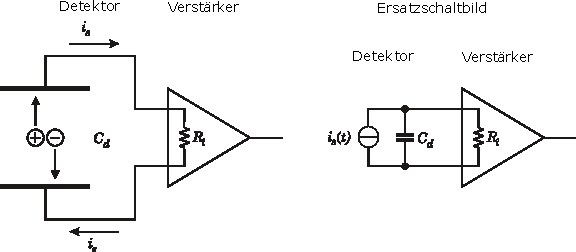
\includegraphics[scale=1.25]{./fig/RamoEquivalent.pdf}
\end{center}
\vspace{-0.5cm}
\caption{Links: Ladungsträger welche sich im Detektorvolumen bewegen erzeugen einen Strom im Schaltkreis. Rechts: Ersatzschaltbild der Schaltung Links. Der Detektor kann als Kapazität mit paralleler, zeitabhängiger Stromquelle dargestellt werden.\cite{Editors}}
\label{fig:RamoEq}
\end{figure}

Für ein qualitatives Verständnis betrachte man eine Ladung $q$ welche sich in der Mitte zwischen zwei unendlich großen Elektroden befindet, wie in der Abbildung \ref{fig:RamoQual} Links dargestellt.
Die Hälfte der Feldlinien terminieren auf der obere und die andere Hälfte auf der Unteren Elektrode.
Integriert man nun den Gaußschen Satz über eine Fläche $S_1$ welche die obere Elektrode umschließt oder eine Fläche $S_2$ welche die untere Elektrode umschließt ergibt sich
\begin{equation}
\oint_{S_1} \vec{E} \,d\vec{a} = \oint_{S_2} \vec{E} \,d\vec{a} = -\frac{q}{2}.
\end{equation}
Das heißt auf beiden Elektroden wird die gleiche Ladung von $-q/2$ induziert.
Befindet sich die selbe Ladung nun in unmittelbarer Nähe zur unteren Elektrode wie in Abbildung \ref{fig:RamoQual} Rechts dargestellt terminiert der Großteil der Feldlinien an der unteren Elektrode.
Die Induzierte Ladung ist somit in der unteren Elektrode deutlich größer.
Eine Ladung die sich also von der oberen zur unteren Elektrode bewegt induziert eine abnehmende Ladung in der oberen Elektrode und eine zunehmende Ladung in der unteren Elektrode.\cite{Editors}

\begin{figure}[!b]
\begin{center}
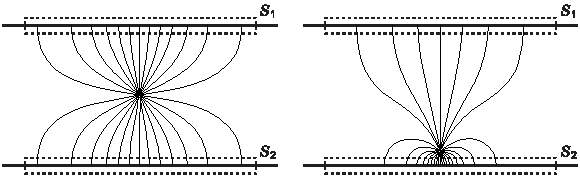
\includegraphics[scale=1.25]{./fig/RamoQual.pdf}
\end{center}
\vspace{-0.5cm}
\caption{Links: Eine Ladung $q$ in der Mitte zwischen zwei Elektroden induziert die gleiche Ladung in beiden Elektroden. Aus dem Gaußschen Satz folgt, dass die Flächen $S_1$ und $S_2$ jeweils die Ladung $-q/2$ einschließen. Rechts: Befindet sich die Ladung in der Nähe der unteren Elektrode terminiert der Großteil der Feldlinien an dieser Elektrode. Daher ist die Ladung welche von $S_2$ eingeschlossen ist größer als die Ladung welche von $S_1$ eingeschlossen ist. \cite{Editors}}
\label{fig:RamoQual}
\end{figure}

Quantitativ wird dieser Effekt durch das Shockley-Ramo-Theorem beschrieben.
Shockley hat diesen Effekt als erstes im Jahr 1938 beschrieben.
Ramo veröffentlichte allerdings eine deutlich elegantere Formulierung im Jahr 1939.
Der durch eine sich mit der Geschwindigkeit $\vec{v}$ bewegten Ladung $q$ erzeugte instantane Strom ist gegeben durch
\begin{equation}
i_k = -q\vec{v}\vec{E}_Q.
\label{eq:RamoCurrent}
\end{equation}
Das \textit{weighting field} $\vec{E}_Q$ unterscheidet sich entscheidend vom Elektrischen Feld zwischen den Elektroden.
Während das \textit{weighting field} die Induzierte Ladung bestimmt ist es das elektrische Feld welches die Dynamik der Ladungsträger diktiert.
$\vec{E}_Q$ erhält man indem die Ladung $q$ entfernt wird, die gegebene Elektrode auf das Potential $1$ gesetzt wird und alle anderen Leiter geerdet werden.\cite{Ramo1939}
Die durch eine Ladung $q$ welche sich von $x_1$ zum Zeitpunkt $t_1$ nach $x_2$ zum Zeitpunkt $t_2$ bewegt Induzierte Ladung ergibt sich aus der Integration des Stroms $i_k$ über die Zeit
\begin{align}
\Delta Q_k &= \int_{t_1}^{t_2}i_k \,dt = \frac{1}{|\vec{v}|} \int_{\vec{r}_1}^{\vec{r}_2}i_k \,dr = -\frac{q}{|\vec{v}|} \int_{\vec{r}_1}^{\vec{r}_2}\vec{v}\vec{E}_Q \,dr = \frac{q}{|\vec{v}|} \int_{\vec{r}_1}^{\vec{r}_2}\vec{v}\nabla\Phi \,dr \nonumber \\
&= q\left(\Phi(r_2) - \Phi(r_1)\right).
\label{eq:RamoCharge}
\end{align}
Das \textit{weighting potential} $\Phi$ hängt über $\vec{E}_Q = -\nabla\Phi$ mit dem \textit{weighting field} zusammen.
Die Induzierte Ladung $\Delta Q$ ist unabhängig vom zurückgelegten Weg der Ladung $q$ sie ist ausschließlich abhängig vom Anfangs- und Endpunkt.

In Abbildung \ref{fig:RamoDeLight} ist der Fall eines Kristalls zwischen zwei Elektroden dargestellt.
Der Kristall ist hierbei durch Vakuum von den Elektroden getrennt.
Zwischen Elektrode und Kristall fällt bereits ein teil des Potentials ab.
Daher durchlaufen die Ladungsträger im Kristall nur einen Teil des angelegten Potentials.
Um die induzierte Ladung entsprechend dem Ramo-Theorem zu berechnen wird das \textit{weigting potential} bestimmt dieses erhält man indem das Potential $V_0$ auf $1$ gesetzt wird.
Ein Event im Detektorvolumen erzeugt eine bestimmte Anzahl von Elektron-Loch-Paaren $N_{eh}$ in der Höhe $z_0$.
Angenommen das Potential $V_0$ ist positiv dann driften die Elektronen in Richtung der 
Elektrode $A$ und die Löcher in Richtung der Elektrode $B$.
Für die auf der Elektrode $A$ induzierte Ladung $\Delta Q$ ergibt sich somit nach Gleichung \eqref{eq:RamoCharge}
\begin{align}
\Delta Q &= e N_{eh}(\Phi(g) - \Phi(z_0)) + (-e)N_{eh}(\Phi(h+g) - \Phi(z_0)) \nonumber \\
&= eN_{eh}\left(b - \Phi(z_0) - a + \Phi(z_0)\right) \nonumber \\
&= -eN_{eh}(a-b).
\label{eq:RamoCharge}
\end{align}
Diese ist unabhängig von der genauen Position $z_0$ des Events.
$(a-b)$ gibt den von den Ladungsträgern durchlaufenen Protzen teil des Gesamten Potentials an.
Entsprechend wird auf der Elektrode $B$ die Ladung $\Delta Q = eN_{eh}(a-b)$ induziert.



\begin{figure}[]
\begin{center}
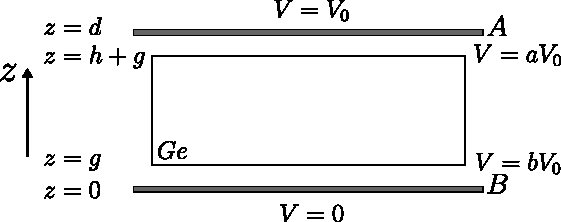
\includegraphics[scale=1.25]{./fig/ElektrodenDeLight.pdf}
\end{center}
\vspace{-0.5cm}
\caption{Anordnung der Elektroden im DeLight Experiment. Annahme eines Homogenen Feldes in x- und y-Richtung. Zwischen Elektrode und Ge-Kristall fällt das Potential von $V_0$ auf $aV_0$ und von $bV_0$ auf $0$ ab, mit $0 < b < a < 1$.}
\label{fig:RamoDeLight}
\end{figure}
	\section{Luke-Verstärkung}\label{sec:LukeAmp}
	Die Fähigkeit Ionisationssignale einzelner Elektronen zu messen ist für die Suche nach leichter Dunkler Materie von großem Interesse.
Das Rauschen in der Ladungsbestimmenden Ausleseelektronik limitiert allerdings die Energieauflößung auf die Größenordnung von $\SI{100}{\electronvolt}$.
Da das Ionisations- und Phononsignal nicht unabhängig ist, ist es möglich die Phononen zu bestimmen welche entstehen wenn Ladungsträger im Kristall driften.
Die Energie der Phononen ist proportional zur angelegten Driftspannung $V_b$ und werden als Luke-Phononen bezeichnet.
Das gesamte Phononsignal setzt sich dann aus dem der initialen Wechselwirkung und der Luke-Phononen zusammen
\begin{equation}
E_P = \frac{E_{dep}}{\epsilon}eV_b + E(1-\frac{\delta}{\epsilon})
\end{equation}
$V_b$ ist die durchlaufene Spannung der Ladungsträger, $e$ die Elementarladung, $\delta$ die minimale Ionisationsenergie und $\epsilon$ die mittlere Energie um eine Elektron-Loch-Paaren zu erzeugen.
Die Konstante $\epsilon$ ist abhängig davon welches Material verwendet wird und ob es sich um Elektron- oder Nukleonstreuung handelt.
Für Elektronstreuung an einem Germaniumkristall ist $\epsilon=\SI{3}{\electronvolt}$\cite{Luke1988}.
Die Anzahl der Elektron-Loch-Paare ist gegeben durch
\begin{equation}
N_{eh} = \frac{E_{dep}}{\epsilon}.
\end{equation}

Der bisherige Ansatz bei EDELWEISS war das initiale Phononsignal nicht zu maskieren indem Biasspannungen in der Größenordnung von $\SI{1}{\volt}$\cite{Arnaud2016} angelegt werden.
Dadurch ist es möglich aus dem gemessenen Phonon- und Ionisationssignal das Phononsignal der ursprünglichen Wechselwirkung zu berechnen.

Alternativ kann durch große Driftspannung die Anzahl von Luke-Phononen pro driftendem Ladungsträger nahezu beliebig groß gewählt werden.
Das rauschen der Ausleseelektronik für das Phononsignal bleibt dabei allerdings unverändert.
Dadurch wird das Signal zu Rausch Verhältnis besser umso höher die Driftspannung ist.
Dabei geht jedoch die Information über das initiale Phononsignal verloren.
Die Absicht ist es auf diese weise einzelne Elektron-Loch-Paare in Germanium auflösen zu können\cite{Mirabolfathi2015}.

	\section{HEMT Übersicht}
	\acp{HEMT} gehören zur Klasse der Feldeffekttransistoren, unterscheiden sich allerdings in ihrem Funktionsprinzip entscheidend von \acsp{JFET} und \acsp{MOSFET}.
Das Funktionsprinzip basiert auf einer Heterostruktur zweier Halbleiter mit unterschiedlich großen Bandlücken.
An der Grenzschicht zwischen einem stark n-dotierten Halbleiter mit großer Bandlücke (z.B. AlGaAs) und einem undotierten Halbleiter mit kleinerer Bandlücke (z.B. GaAs) kommt es zum band bending und es entsteht eine Struktur, wie sie in Abb. \ref{fig:HEMTBand} dargestellt ist.
Elektronen aus dem n-dotierten Material diffundieren in das Leitungsband auf der Seite des undotierten Materials.
Dadurch entsteht entlang der Grenzfläche ein 2D-Elektronengas.
Durch eine Spannung am Gate kann die Anzahl der Elektronen im Leitungsband beeinflusst werden.
Da sich die Leitungselektronen auf Seiten des undotierten GaAs befinden, kommt es seltener zu Coulomb-Streuung, was zu einer hohen Mobilität der Elektronen führt.
Daher stammt auch der Name von Transistoren dieser Art.\cite{HEMTFundamental, Mimura2002}

\begin{figure}[!b]
\begin{center}
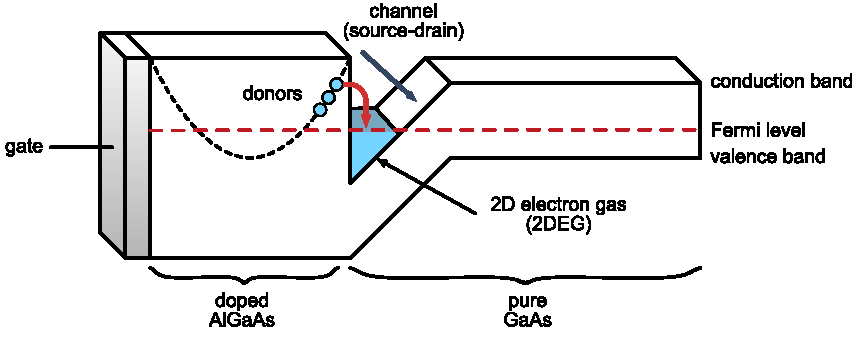
\includegraphics[scale=1]{./fig/HEMTBand.pdf}
\vspace{-0.5cm}
\caption{Bandstruktur eines typischen HEMTs.
Elektronen aus dem stark n-dotierten AlGaAs diffundieren in das undotierte GaAs und bilden dort ein 2D-Elektronengas.
Über die Gatespannung wird die Lage des Fermilevel und damit die Menge an Elektronen im Leitungsband variiert.\cite{Thomas2016}}
\label{fig:HEMTBand}
\end{center}
\end{figure}

Bisherige niederfrequente kryogene Verstärkerelektroniken basieren vorwiegend auf JFETs.
Die Technik von JEFTs stößt allerdings an zwei für diesen Anwendungsbereich entscheidende Grenzen.
Erstens frieren JFETs unter einer Temperatur von $\SI{100}{\kelvin}$ ein und werden idealerweise bei einer Temperatur von $\SI{130}{\kelvin}$ verwendet.
Daher ist entweder eine Heizung im Krysotaten notwendig oder lange Kabel zwischen Ausleseelektronik und Detektor, welche Auslesegeschwindigkeit und Signalqualität verringern.
Zweitens liegt das minimal mögliche Rauschen in der Größenordnung von $\SI{1}{\nano\volt\per\sqrt\hertz}$ bei einer Frequenz von $\SI{1}{\kilo\hertz}$\cite{HEMTYang2011}.
HEMTs und MOSFETs hingegen funktionieren selbst bei kryogenen Temperaturen.
Diese Arten von Transistoren wurden bisher allerdings nicht verwendet aufgrund ihres hohen niederfrequenten $1/f$-Rauschen.

Infolge aktueller Entwicklungen des \ac{CNRS} an der Universität Paris-Süd ist es gelungen HEMTs zu entwerfen, welche vielversprechende Eigenschaften aufweisen im Gegensatz zu handelsüblichen HEMTs.
Die Erste dieser Eigenschaften ist ein hervorragendes $1/f$-Rauschen von $\SI{0.46}{\nano\volt\per\sqrt\hertz}$ bei einer Frequenz von $\SI{1}{\kilo\hertz}$ und einer Temperatur von $\SI{4.2}{\kelvin}$.
Die Eingangskapazität liegt in der Größenordnung von $\SI{100}{\pico\farad}$, womit sie gut an die Detektorkapazität angepasst ist.
Zweitens liegt ihre benötigte Leistung in der Größenordnung von $\SI{30}{\mu\watt}$ deutlich unter der von JFETs.\cite{HEMTYang2011}
Dadurch ist es möglich eine größere Anzahl von Ionisationskanälen im Kryostaten zu installieren.
Zuletzt sind diese HEMTs zur Anwendung bei kryogenen Temperaturen ausgelegt.
Werden JFETs im Kryostaten verwendet, ist es notwendig eine Heizung einzubauen.
Diese erzeugt Schwarzkörperstrahlung, welche wiederum vom Detektor absorbiert werden kann.
Außerdem muss sie von der restlichen Anordnung isoliert werden. 
Die dazu verwendete Membran erzeugt zusätzliches niederfrequentes Rauschen durch ihre Schwingungen.





	\section{Rauschen}\label{sec:Rauschen}
	Elektrisches Rauschen stammt im Wesentlichen daher, dass elektrische Ladung nicht kontinuierlich verteilt ist und daher statistische Effekte der Ladungsträger zu Rauschen führen.
Rauschen wird in der Regel als Varianz einer Strom- oder Spannungsquelle normiert auf das Frequenzband angegeben, die Einheit ist dann $\SI{}{\ampere^2\per\sqrt\hertz}$ bzw. $\SI{}{\volt^2\per\sqrt\hertz}$.
Das minimal messbare Signal ist maßgeblich durch das vorhandene Rauschen bestimmt.
Nur wenn sich das Signal signifikant vom statistischen Rauschen unterschiedet, kann es gemessen werden.\cite{Gray}

\subsection*{Schrotrauschen}
Schrotrauschen tritt immer dann auf, wenn ein Strom durch einen n-p-Übergang fließt, wie es zum Beispiel bei Bipolartransistoren der Fall ist.
Begründet liegt das Rauschen in der statistischen Verteilung der Energie und Geschwindigkeit der Elektronen.
Nur wenn die Energie groß genug ist und die Geschwindigkeit in Richtung des Übergangs zeigt, kann die Barriere überquert werden.
Daher ist der externe Strom aus vielen zufälligen Pulsen zusammengesetzt.
Die Varianz auf den Strom ist für Shot Noise gegeben durch
\begin{equation}
\stackrel{-}{i}^2 = 2eI.
\end{equation}
Diese Art von Rauschen ist unabhängig von der Frequenz und gehört daher dem weißen Rauschen an.
Im Ersatzschaltbild wird diese Rauschen durch eine Stromquelle parallel zum Widerstand $r_d = \frac{k_BT}{eI}$ des p-n-Übergangs dargestellt.

\begin{figure}[!t]
\begin{center}
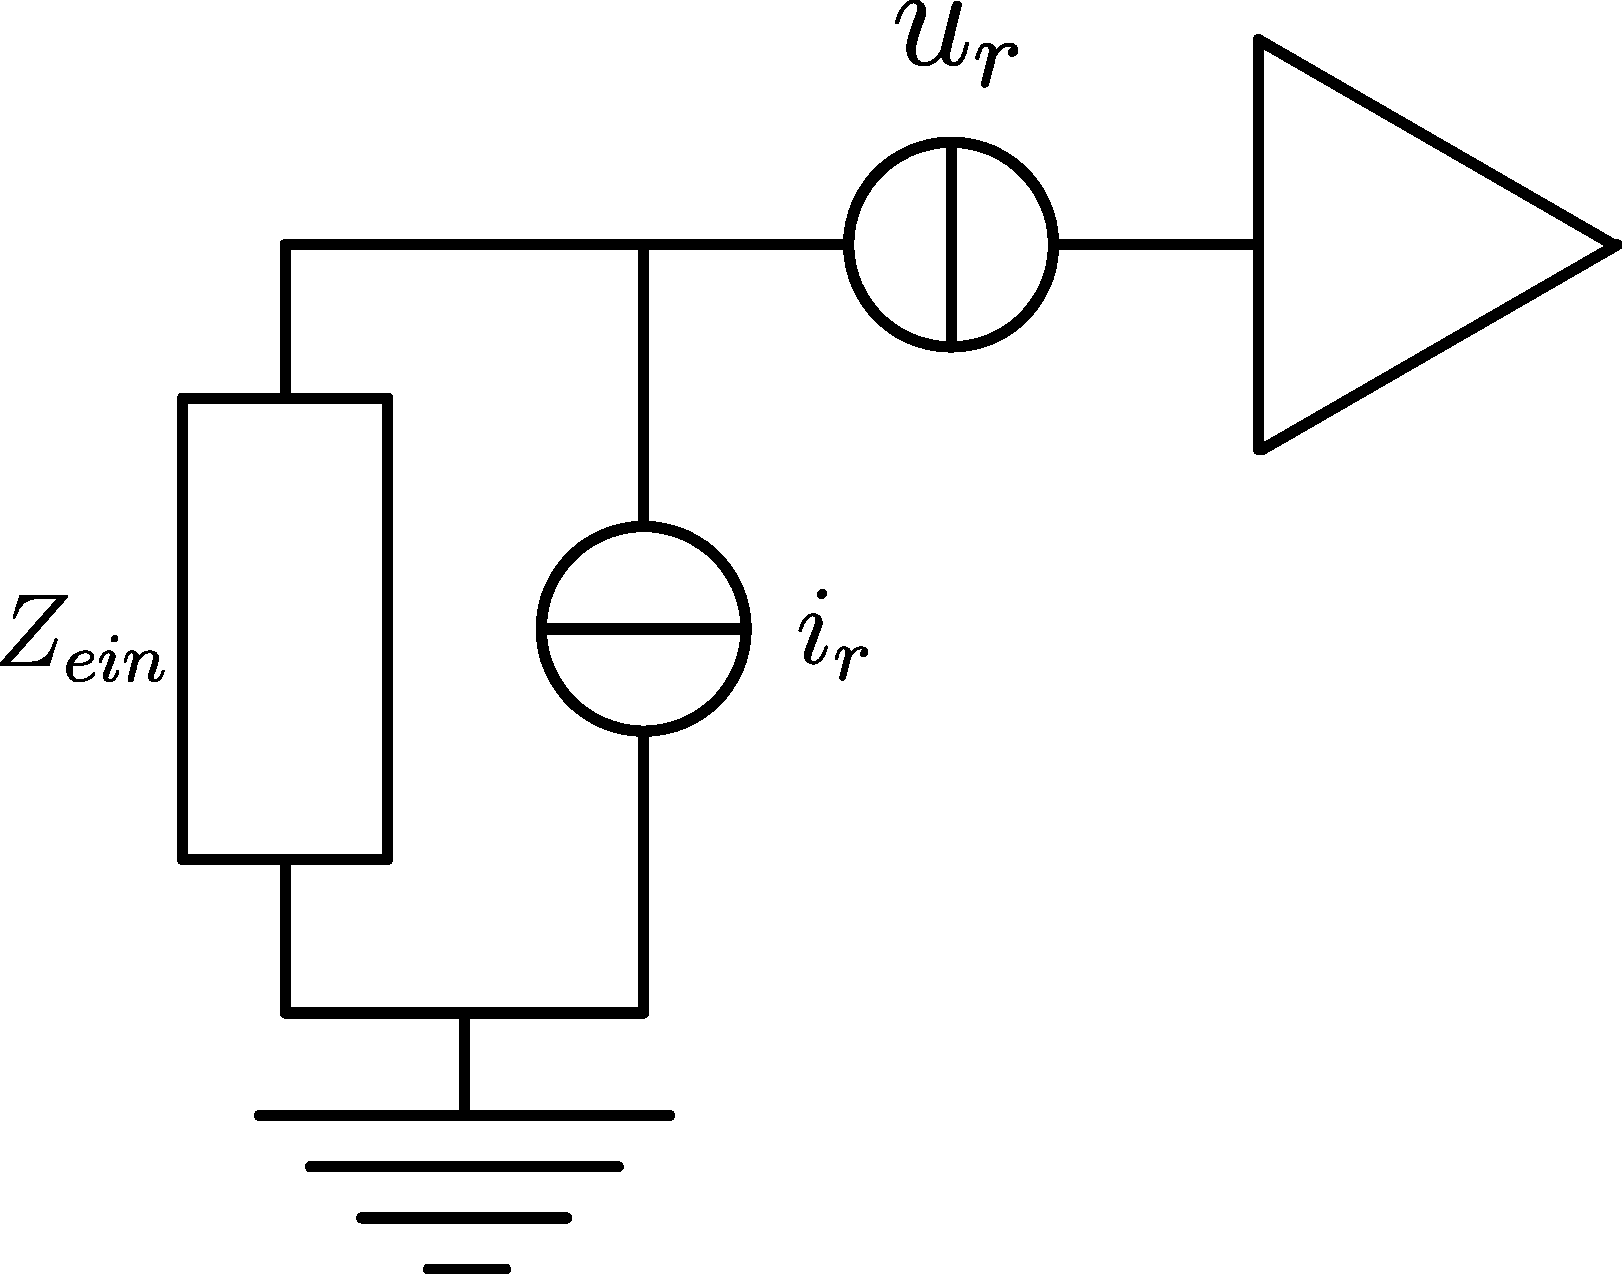
\includegraphics[width=0.50\textwidth]{./fig/NoiseSchematic.pdf}
\vspace{-0.5cm}
\caption{Ersatzschaltbild des Verstärkers.
Das Rauschen des Verstärkers wird in Form einer Rauschstromquelle $i_r$ parallel zur Eingangsimpedanz und einer Rauschspannungsquelle $u_r$ in Reihe zum Eingang eines idealen Verstärkers modelliert.
Der ideale Verstärker selbst ist frei von Rauschen.
Indem das Rauschen eingangsseitig betrachtet wird, können verschiedene Verstärker leichter verglichen werden, ohne dass die individuellen Übertragungsfunktionen berücksichtigt werden müssen.}
\label{fig:NoiseSchematic}
\end{center}
\end{figure}

\subsection*{Wärmerauschen}
Wärmerauschen entsteht in Widerständen durch die zufällige thermische Bewegung der Elektronen und ist somit im Gegensatz zum Schrotrauschen unabhängig von einem externen Strom.
Das Wärmerauschen kann im Ersatzschaltbild entweder durch eine Stromquelle parallel zum Widerstand der Größe
\begin{equation}
\stackrel{-}{i}^2 = \frac{4k_B T}{R}
\end{equation}
oder eine Spannungsquelle in Reihe zum Widerstand dargestellt werden.

\subsection*{1/f-Rauschen}
1/f-Rauschen tritt sowohl in passiven als auch in aktiven Elementen auf und liegt in vielen Ursachen begründet.
Unter anderem in der fluktuierenden Beweglichkeit der Ladungsträger.
In FETs wird 1/f-Rauschen üblicherweise als Spannungsquelle am Eingang modelliert
\begin{equation}
\stackrel{-}{e}^2 = \frac{K}{f^b}.
\end{equation}
Der Parameter $K$ ist abhängig vom Bauteil und eine Funktion des Stroms.
Der Parameter $b$ liegt in der Regel nahe bei $1$, daher der Name dieser Rauschart.

\subsection*{Verstärker Rauschen}
Das Rauschen des Verstärkers wird wie in Abb. \ref{fig:NoiseSchematic} durch die eingangsseitige Spannungsquelle $u_r$ in Reihe zum Verstärker und einer eingangsseitigen  Stromquelle $i_r$ parallel zur Eingangsimpedanz modelliert.
Die Spannungsquelle wird als ein 1/f-Rauschen und ein konstantes weißes Rauschen modelliert\cite{horowitz1980art}
\begin{equation}
u^2_r = \frac{A^2}{f} + u^2_w.
\end{equation}
Parallel zur Eingangsimpedanz ist die Rauschstromquelle $i_r$ deren Rauschen gemäß
\begin{equation}
i^2_r = a + bf + cf^2
\end{equation}
modelliert wird\cite{Thomas2016}.
Diese beschreibt den Anteil des Rauschens, welcher von der Eingangsimpedanz abhängig ist und führt zu dem Spannungsrauschen
\begin{equation}
u^2_{ri} = Z^2_{ein}i^2_r.
\end{equation}
Es wird angenommen, dass die einzelnen Rauscharten unabhängig voneinander sind und werden daher quadratisch addiert.
Das gesamte Rauschen ergibt sich somit aus dem Verstärker Rauschen, welches das thermische Rauschen beinhaltet und dem Schrotrauschen aufgrund des Leckstrom zu
\begin{align}
u_{ges} &= \frac{A^2}{f} + u^2_w + Z^2_{ein}(i^2_r + i_{Schrot}) \\
&= \left(\frac{a + 2eI_{Leck}}{4\pi^2 C^2_{ges}}\right)\frac{1}{f^2} + \left(A^2 + \frac{b}{4\pi^2 C^2_{ges}}\right)\frac{1}{f} + u^2_w + c
\label{eq:Rauschen}
\end{align}
mit $Z_{ein}$ aus Gl. \eqref{eq:EingangsC}.

	
	\chapter{Konzept für Entwurf und Aufbau der Prototyp Verstärkerelektronik}\label{sec:Elektronik}
	Dieses Kapitel beschreibt die Verstärkerelektronik für den Ionisationskanal welche im Rahmen dieser Arbeit entwickelt wurde.
Im Anschluss wird diese dann bei Raumtemperatur und Flüssigstickstoff Temperatur getestet.

	\section{Kalte Elektronik}\label{sec:Ausleseelektronik}
	Der experimentelle Aufbau fordert, dass die Ausleseelektronik für den Ionisationskanal einen sehr kleine Ladung in form eines sehr kleinen und kurzen Strom verstärkt welcher im Kryostaten bei $\sim\SI{20}{\milli\kelvin}$ entsteht.
Damit dieser digitalisiert werden kann ist ein Impedanzwandler notwendig um die Quelle nicht zu belasten.
Dazu werden in der Regel Ladungsverstärker verwendet\cite{Censier2012}.
Diese wandeln ein Ladungsmenge in eine dazu proportionales Spannungssignal um.

Durch die Verwendung von HEMTs ist eine komplette Kryogene Verstärkerelektronik bei $\SI{4}{\kelvin}$ möglich.
Diese hat den Vorteil des niedrigen Rauschen der HEMTs sowie ihr geringer Leistungsverbrauch.
Zusätzlich kann das Signal in unmittelbar nähe zum Detektor ausgelesen werden.
Dadurch ist das Signal weniger anfällig für Störungen durch die langen Kabel aus dem Kryostaten heraus.

Das Schaltbild der Ausleseelektronik ist in Abbildung \ref{fig:Ausleseelektronik} dargestellt und ist eine Form eines Ladungsverstärkers.
Bei einem Event entsteht eine bestimmte Anzahl von Elektron-Loch-Paaren abhängig von der deponierten Energie und dem Detektormaterial.
Bei Germanium Kristallen entsteht ein Elektron-Loch-Paar pro $\sim\SI{3}{\electronvolt}$ deponierter Energie.

\begin{figure}[!t]
\begin{center}
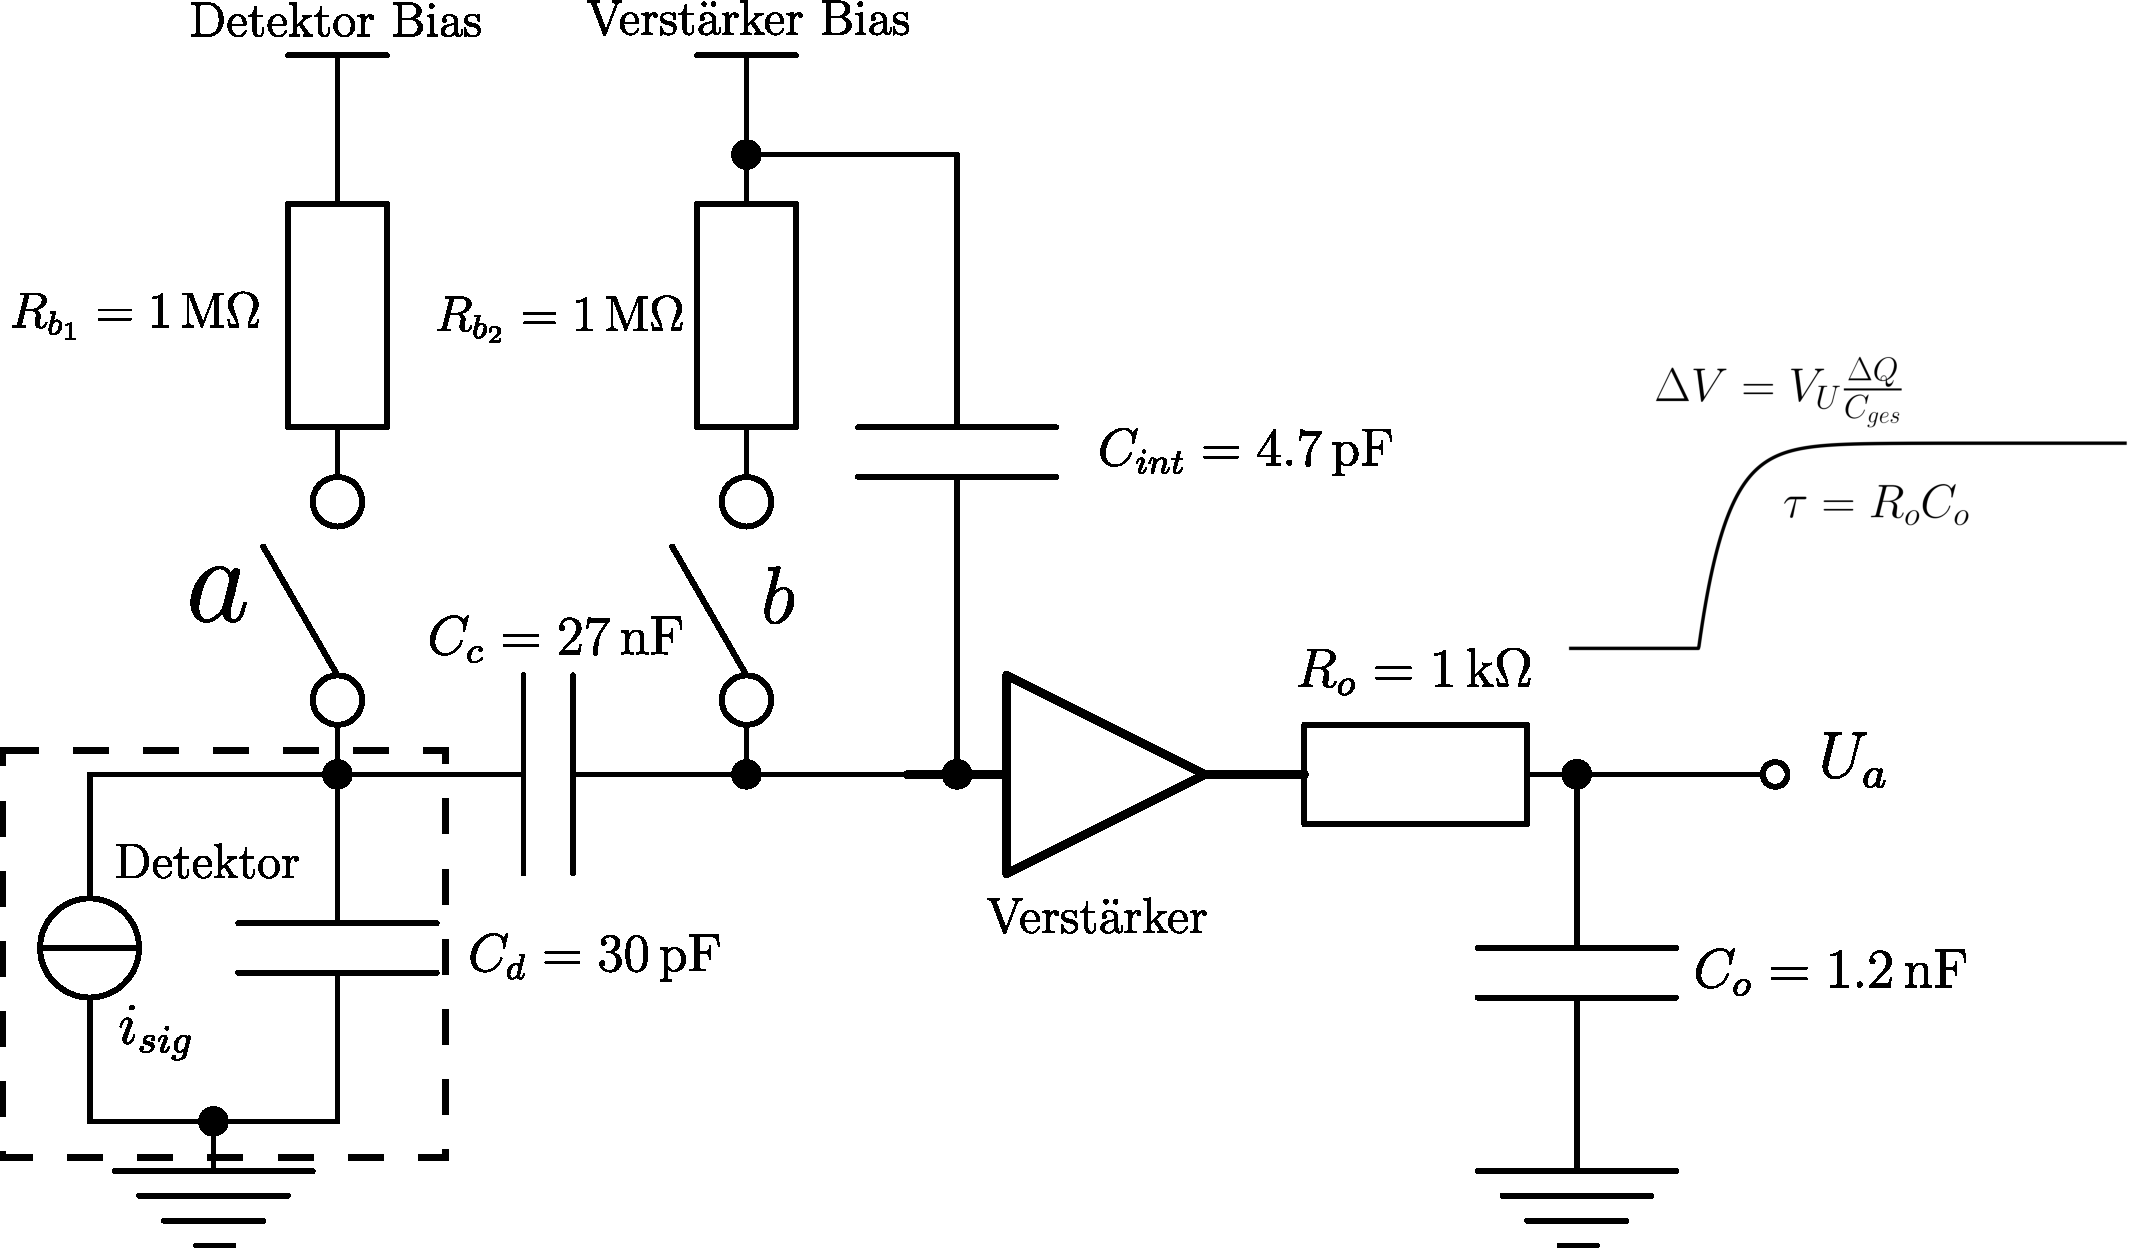
\includegraphics[width=\textwidth]{./fig/Ausleseelektronik.pdf}
\vspace{-0.5cm}
\caption{Das Design der Kalte Elektronik entspricht dem eines Ladungsverstärkers.
Der Detektor ist durch sein Ersatzschaltbild entsprechend dem Ramo-Theorem als Stromquelle parallel zur Detektorkapazität dargestellt.
Der Verstärker ist vereinfacht als Dreieck dargestellt.
Nicht eingezeichnet ist die Versorgungsspannung des Verstärkers und die Spannung zum schalten der Relais.}
\label{fig:Ausleseelektronik}
\end{center}
\end{figure}

Der Detektor wird entsprechend dem Ramo-Theorem im Ersatzschaltbild durch eine Stromquelle parallel zur Detektorkapazität dargestellt.
Der Signalstrom ist nach Gleichung \eqref{eq:RamoCurrent} abhängig von der Driftgeschwindigkeit.
In Germanium beträgt diese abhängig von der angelegten Biasspannung mehrere $\SI{}{\centi\meter}/\SI{}{\micro\second}$\cite{Jacoboni1981}.
Um in einem $\sim\SI{2}{\centi\meter}$ dicken Detektor den genauen Stromverlauf zu verfolgen ist somit ein Verstärker mit einer Bandbreite von mehreren $\SI{}{\mega\hertz}$ notwendig.
Der genaue Verlauf ist allerdings für Energiebestimmung uninteressant.
Weshalb wir uns auf den Bereich zwischen $DC\--\SI{100}{\kilo\hertz}$ beschränken.
Daher wird der Signalstrom als Deltapeak modelliert werden
\begin{equation}
i_{sig}(t) = \Delta Q \delta(t) = -eN_{eh}(a-b)\delta(t).
\end{equation}
$\Delta Q$ ist die Ladung welche gemäß dem Ramo-Theorem Gleichung \eqref{eq:RamoCharge} in der Elektrode induziert wird.

Um den kurzen Signalstrom zu messen wird dieser auf den zur Stromquelle parallelen Kapazität integriert.
Sodass ein stufenförmiges Spannungssignal entsteht.

Die Schalter dienen dazu die Kapazitäten vor zu spannen damit am Detektor und am Eingang des Verstärkers die gewünschten Biasspannungen anliegen.
Im Normalbetrieb sind die Schalter offen.
Dies hat den Vorteil, dass das Rauschen der Spannungsquellen und der Biaswiderstände nicht das Signal verunreinigen.

Da der Detektor und der Verstärkereingang in der Regel auf unterschiedlichen DC Level liegen ist die Koppelkapazität $C_c$ notwendig.
Da die Kapazität $C_c$ das Signal allerdings wider differenziert ist eine weitere Kapazität $C_int$ notwendig welche das Signal am Eingang des Verstärkers integriert.
Die Koppelkapazität belastet das Signal gemäß
\begin{equation}
\frac{U_e}{U_s} = \frac{C_c}{C_c + C_{int}} \stackrel{C_{int} \ll C_c}{\approx} 1.
\end{equation}
Das heißt die Koppeleffizienz geht gegen $1$ wenn die Koppelkapazität deutlich größer gewählt wird als die Kapazität $C_{int}$.

Die Fouriertransformation des Signalstroms ist $i_{sig}(f)=\Delta Q$.
Durch Multiplikation mit der Eingangsimpedanz bei geschlossenen Schalter $a$ und offenem Schalter $b$ erhalten wir das Spannungssignal
\begin{equation}
U_{sig}(f) = i_{sig}(f)Z_{ein} = i_{sig}(R_b||Z_{C_{ges}}) = \Delta Q \frac{R_b}{1 + j2\pi f C_{ges}R_b}.
\label{eq:InitialSig}
\end{equation}
Die Kapazität $C_{ges}$ ist die Gesamtkapazität aus der Detektorkapazität $C_d$, der Koppelkapazität $C_c$, und der Kapazität $C_{int}$ 
\begin{equation}
C_{ges} = C_d + \frac{C_cC_{int}}{C_{int} + C_c} \stackrel{C_{int} \ll C_c}{\approx} C_d + C_{int}.
\end{equation}
Im Zeitraum erhalten wir dann für das Spannungssignal
\begin{equation}
U_{sig}(t) = \frac{\Delta Q}{C_{ges}}e^{-\frac{t}{R_bC_{ges}}}\Theta(t).
\end{equation}
Wie erwartet kommt es also zu einem Sprung dessen Höhe $\Delta Q/C_{ges}$ die relevante Information über die Anzahl der Ladungsträger und damit der deponierten Energie enthält.
Die Stufe fällt allerdings mit der Zeitkonstante $\tau=R_bC_{ges}$ exponentiell ab.
Im normalen betrieb ist jedoch auch der Schalter $a$ geöffnet.
Dies entspricht $R_b\rightarrow\inf$ das heißt
\begin{equation}
U_{sig}(t)\rightarrow U_{sig}(t)=\frac{\Delta Q}{C_{ges}}\Theta(t).
\end{equation}
Da die Stufe somit nicht mehr abklingt ist es notwendig das DC Level in bestimmten Zeitintervallen durch schließen der Schalter zurückzusetzen.

Durch einen Tiefpass am Ausgang des Verstärkers wird das Frequenzband auf den interessanten Bereich $DC \-- \SI{100}{\kilo\hertz}$ eingeschränkt.
Dies verbessert das Signal zu Rausch Verhältnis und verhindert gleichzeitig, dass hochfrequente Schwingungen über die langen Kabel auf den Eingang des Verstärkers Rückkoppeln wodurch der Verstärker anfangen kann zu oszillieren.
Die Grenzfrequenz ist gegeben durch 
\begin{equation}
f_{-3\,\mathrm{db}} = \frac{1}{2\pi R_o C_o}
\end{equation}

Die Form des Signals nach dem Verstärker und dem Tiefpass lässt sich am einfachsten bestimmen wenn wir wieder von Gleichung \eqref{eq:InitialSig} ausgehen und zum Schluss  den Widerstand $R_b$ gegen unendlich gehen lassen um das verhalten bei offenem Schalter zu erhalten.
Indem wir also Gleichung \eqref{eq:InitialSig} mit der Übertragungsfunktion des Verstärkers $\alpha(f)$ und des Tiefpass multiplizieren erhalten wir
\begin{equation}
U_{sig}(f) = \Delta Q \frac{R_b}{1 + j2\pi f C_{ges}R_b} \alpha(f) \frac{1}{1 + j 2 \pi f C_o R_o}.
\end{equation}
Der Verstärker verhält sich auch wie ein Tiefpass dessen Grenzfrequenz allerdings deutlich größer ist.
Daher kann die Übertrangungsfunktion des Verstärkers als konstant angenommen werden $\alpha(f) = V_U$ in dem von uns betrachteten Frequenzband.
Durch die Rücktransformation erhalten wir schließlich
\begin{equation}
U_{sig}(t) = V_U \frac{\Delta Q}{C_{ges}}(1 - e^{-t/R_oC_o}).
\end{equation}
In der Abbildung \ref{fig:Ausleseelektronik} ist die Form des Ausgangssignals rechts im Bild dargestellt.

	\section{Verstärker}\label{sec:Amp}
	Die Anforderungen an den Verstärker sind eine hohe Eingangsimpedanz damit das Signal nicht belastet wird und eine möglichst große Spannungsverstärkung nah am Detektor um ein optimales Signal zu Rausch Verhältnis zu gewährleisten.
Für den Verstärker wird die Schaltung wie sie in Abbildung \ref{fig:Amp} links dargestellt ist verwendet, Sourceschaltung\cite{Tietze2002} genannt.
In dieser Schaltung wird das Gate des HEMT $T$ als Eingang verwendet.
In das Gate fließt fast kein Strom daher wird der Eingangswiderstand als unendlich angesehen.
Wie bei FETs müss allerdings auch bei HEMTs die parasitären Gate-Drain und Gate-Source Kapazitäten berücksichtigt werden.
Da es sich bei der Sourceschaltung zusätzlich um einen invertierenden Verstärker handelt muss der Millereffekt berücksichtigt werden.
Dieser beschreibt die effektive Vergrößerung der Gate-Drain Kapazität aufgrund der Spannungsverstärkung $V_U$
\begin{equation}
C_M = (1+ |V_U|)C_{gd}.
\end{equation}
\begin{minipage}[!b]{\textwidth}
\begin{minipage}[c]{0.4\textwidth}
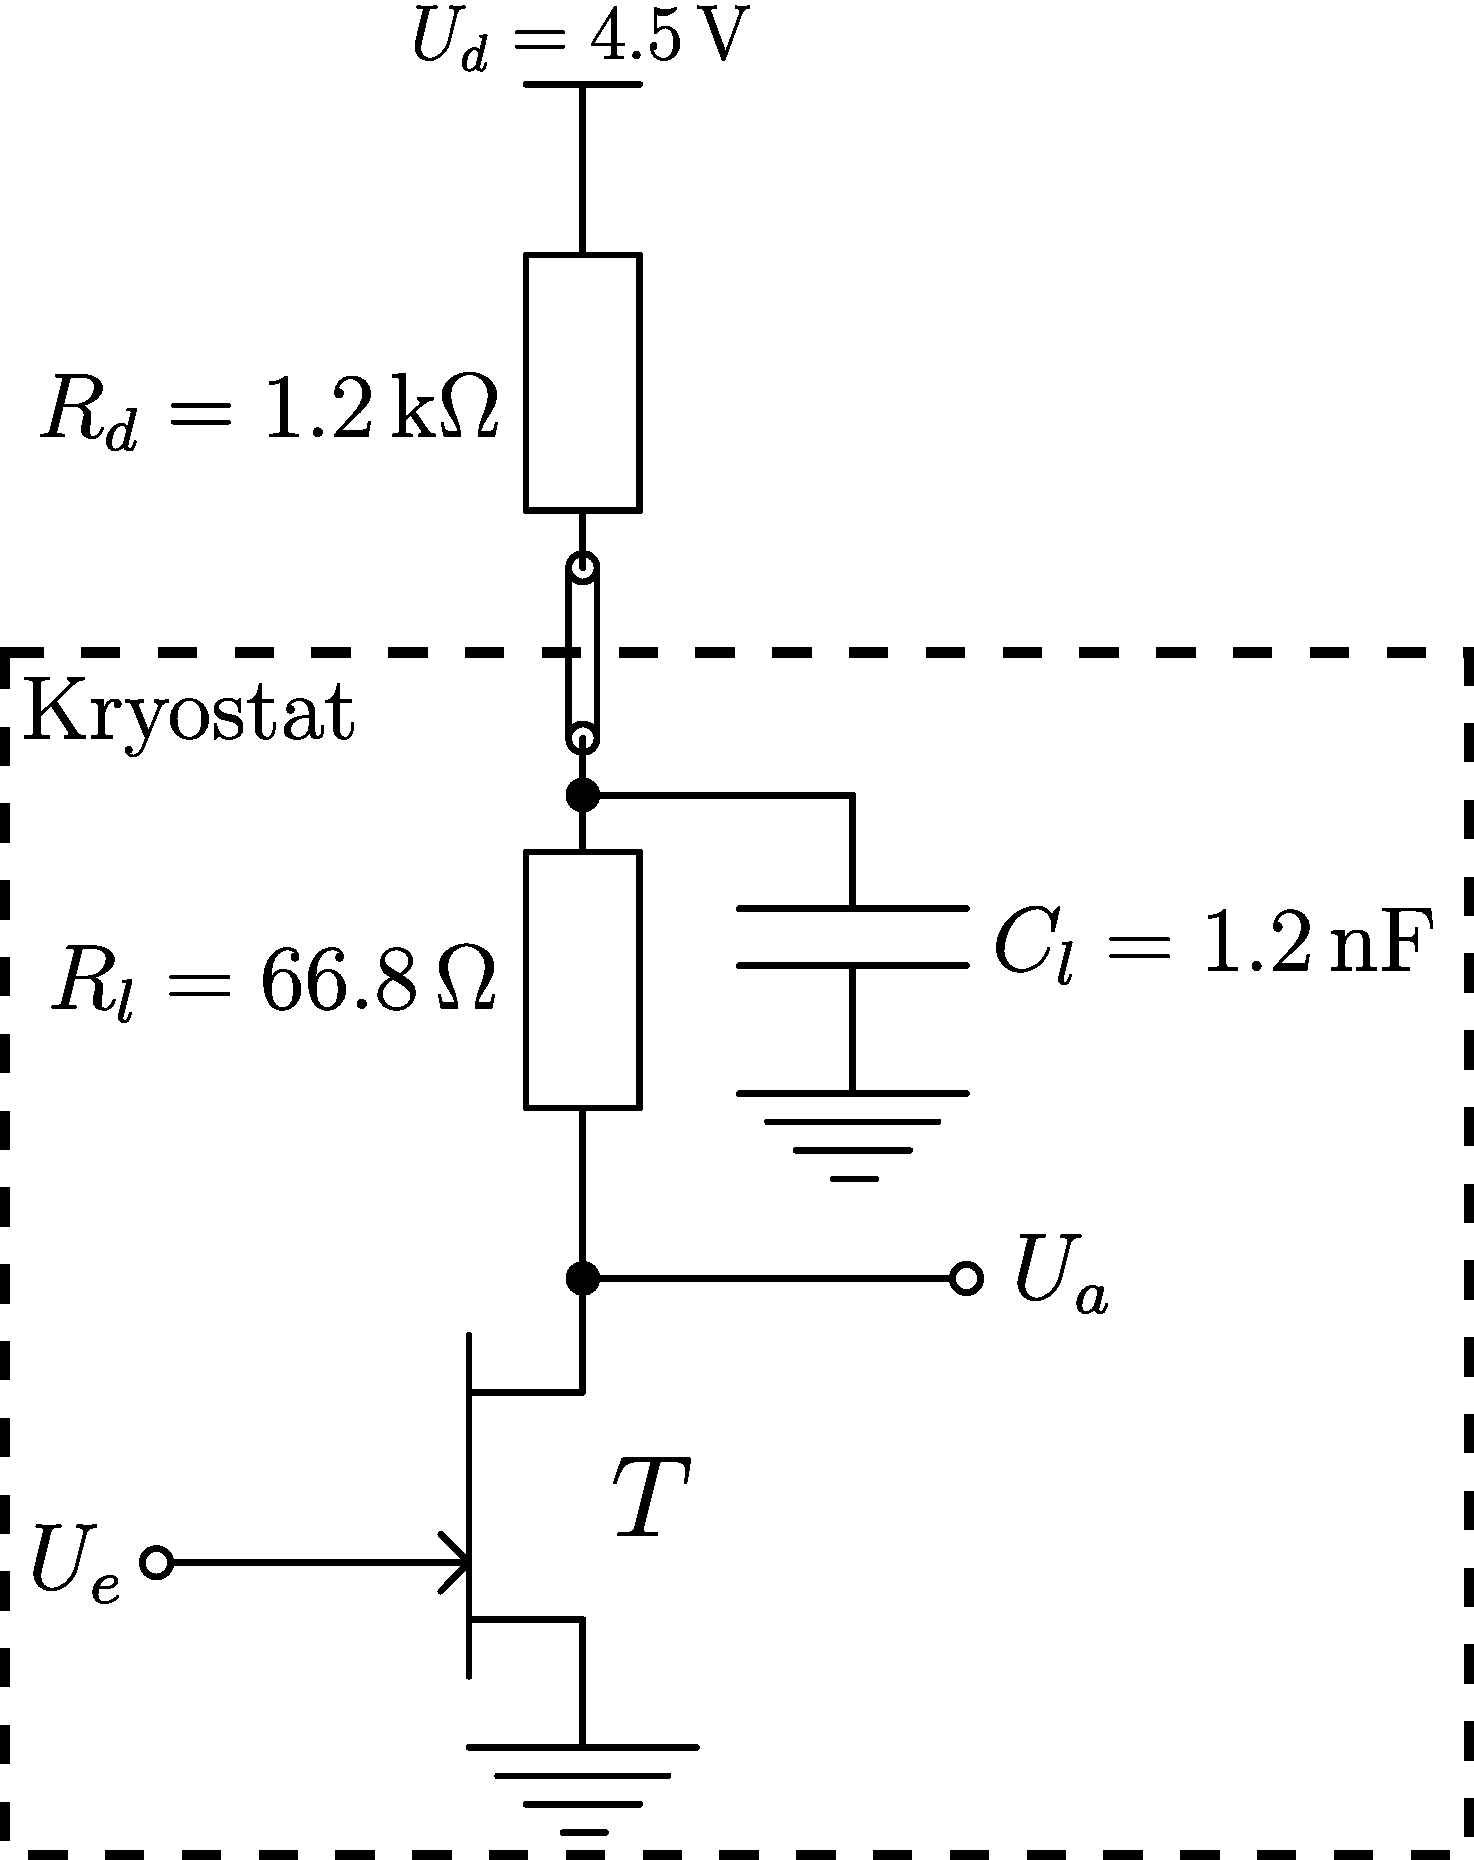
\includegraphics[width=0.9\textwidth]{./fig/Amp.pdf}
\end{minipage}
\begin{minipage}[c]{0.6\textwidth}
\begin{minipage}[c]{0.5\textwidth}
  \begin{tabular}{cc} \toprule
  Eingangskapazität & $\SI{127}{\pico\farad}$ \\ 
  Ausgangswiderstand ($\SI{10}{\kilo\hertz}$) & $\SI{1167}{\ohm}$ \\
  Transkonduktanz & $\SI{410}{\milli\siemens}$\\
  Grenzfrequenz Tiefpass & $\SI{1.99}{\mega\hertz}$\\
  Gate Leckstrom & $\sim\SI{1}{\micro\ampere}$ \\
  Leistung im Warmen &  $\SI{4.1}{\milli\watt}$\\
  Leistung im Kryostat &  $\SI{4.5}{\milli\watt}$\\ \bottomrule
 	\end{tabular}
\end{minipage} \\
\begin{minipage}[c]{0.5\textwidth}
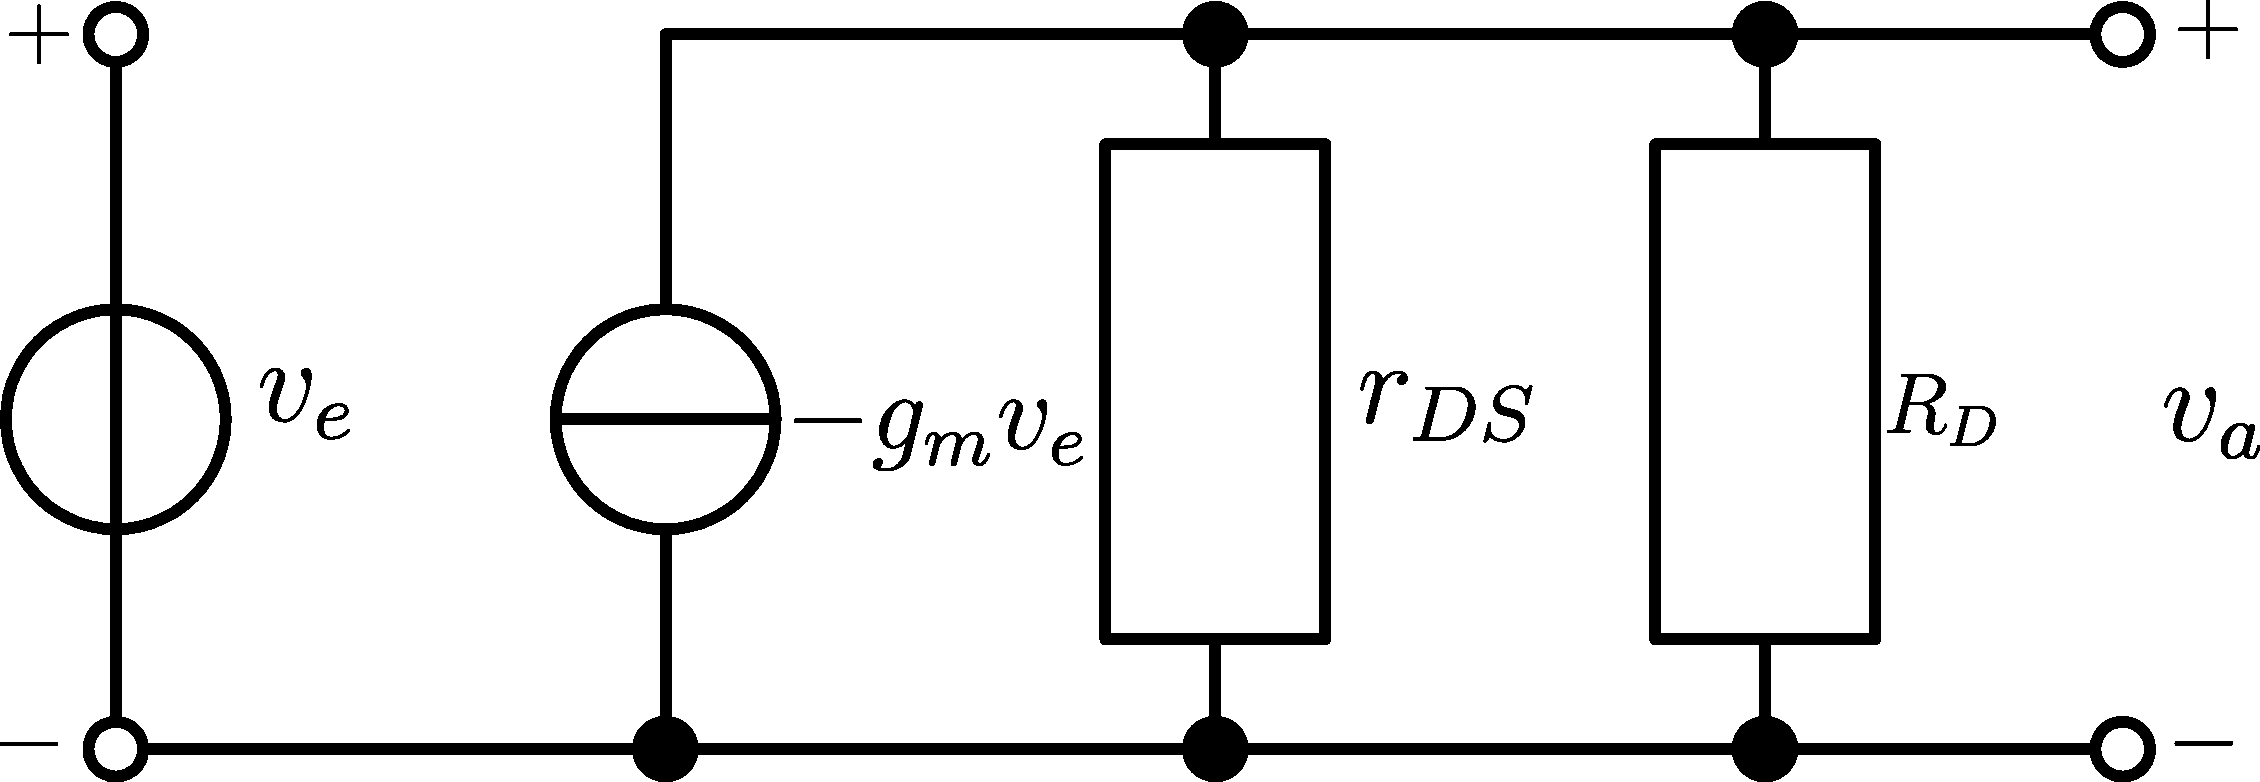
\includegraphics[width=2\textwidth]{./fig/AmpEq.pdf}
\end{minipage}
\end{minipage}
\captionof{figure}{Links: Schaltbild des Verstärkers mit Aufteilung in Raumtemperatur und Kryostat Anteil. Rechts oben: Wichtige Parameter berechnet aus den Angaben im Datenblatt zu dem handelsüblichen HEMT ATF-54143\cite{ATF-54143}. Rechts unten: Ersatzschaltbild des links dargestellten Verstärkers.}
\label{fig:Amp}
\end{minipage}
\vspace{1mm}
Für die Eingangskapazität gilt also $C_e = C_{gs} + C_M$.

Das Ersatzschaltbild ist in Abbildung \ref{fig:Amp} rechts unten dargestellt.
Der Transistor wird durch eine spannungsgesteuerte Stromquelle ersetzt.
Dieser wandelt die Eingangspannung mittels der Transkonduktanz $g_m$ in einen dazu proportionalen Strom.
Für die Spannungsverstärkung ergibt sich
\begin{equation}
V_U = \frac{v_a}{v_e} = -\frac{(r_{DS}||R_D)g_mv_e}{v_e} = -(r_{DS}||R_D)g_m \approx
-g_m R_D.
\end{equation}
Der Widerstand $R_D$ ist eine Kombination aus den Widerständen und Kapazitäten $R_d$, $R_l$, $C_l$ und daher Frequenzabhängig.
In dem interessanten Bereich $\text{DC} \-- \SI{10}{\kilo\hertz}$ ist er allerdings nahezu konstant.
\begin{equation}
R_D = R_l + \frac{R_d}{1 + 2\pi R_d C_l f} \approx R_l + R_d
\end{equation}
Die Verstärkung hängt somit entscheidend von der Transkonduktanz, welche in der Regel stark Temperaturabhängig ist, und dem Drainwiderstand $R_D$ ab.
Um die Abhängigkeit der Verstärkung von der Transkonduktanz und dadurch von der Temperatur aufzuheben wird oftmals ein teil des Ausgangssignal auf den Eingang rückgekoppelt.
Auf kosten einer kleineren Verstärkung wird diese dadurch stabilisiert.
Aufgrund der nur sehr kleinen Temperaturschwankungen im Kryostaten ist dies hier nicht notwendig und birgt eher das Risiko, dass der Verstärker anfängt zu schwingen.
Durch das vergrößern des Widerstand $R_D$ kann die Verstärkung nicht beliebig groß gewählt werden, da man sonst an den Rand des Ausgangskennlinienfeld gerät, d.h. am Transistor fällt eine zu kleiner Spannung ab und es fließt ein zu kleiner Strom.

Der Ausgangswiderstand ist gegeben durch
\begin{equation}
R_a = \frac{u_a}{i_a} = r_{DS}||R_D \approx R_D.
\end{equation}
Der Großteil des Drainwiderstand ist außerhalb des Kryostat dadurch wird die Leistung welche innerhalb des Kryostaten verbraucht wird minimiert.
Die Leistung spielt eine entscheidende Rolle dabei wie viele Detektoren im Kryostaten betrieben werden können.

Die Kombination aus $R_l$ und $C_l$ bildet zusammen einen Tiefpass mit der Grenzfrequenz
\begin{equation}
f_{-3\,\mathrm{db}} = \frac{1}{2\pi R_l C_l}
\end{equation}
Dadurch bleibt der interessante Frequenzbereich unbeeinflusst aber es wird verhindert, dass hochfrequente Schwingungen über die Kabel zurück auf den Eingang des Verstärkers koppeln.
Die Größe der Grenzfrequenz ist durch die verfügbaren Kapazitäten und durch die Leistung welche im Kryostat verbraucht werden soll begrenzt.


	\section{Experimenteller Aufbau}
	Das Ziel des Versuchsaufbaus ist es die Verstärkung und das Rauschen der Elektronik aufzunehmen unter möglichst ähnlichen Bedingungen wie sie beim Einsatz im Kryostaten mit einem Detektor gegeben sind.
Dazu wird die kalte Elektronik wie sie in den Abschnitten \ref{sec:Ausleseelektronik} und \ref{sec:Amp} dargestellt ist verwendet.
Für den Verstärker wurde eine Auswahl verschiedener handelsüblicher HEMTs verwendet.

\begin{figure}[!t]
\begin{center}
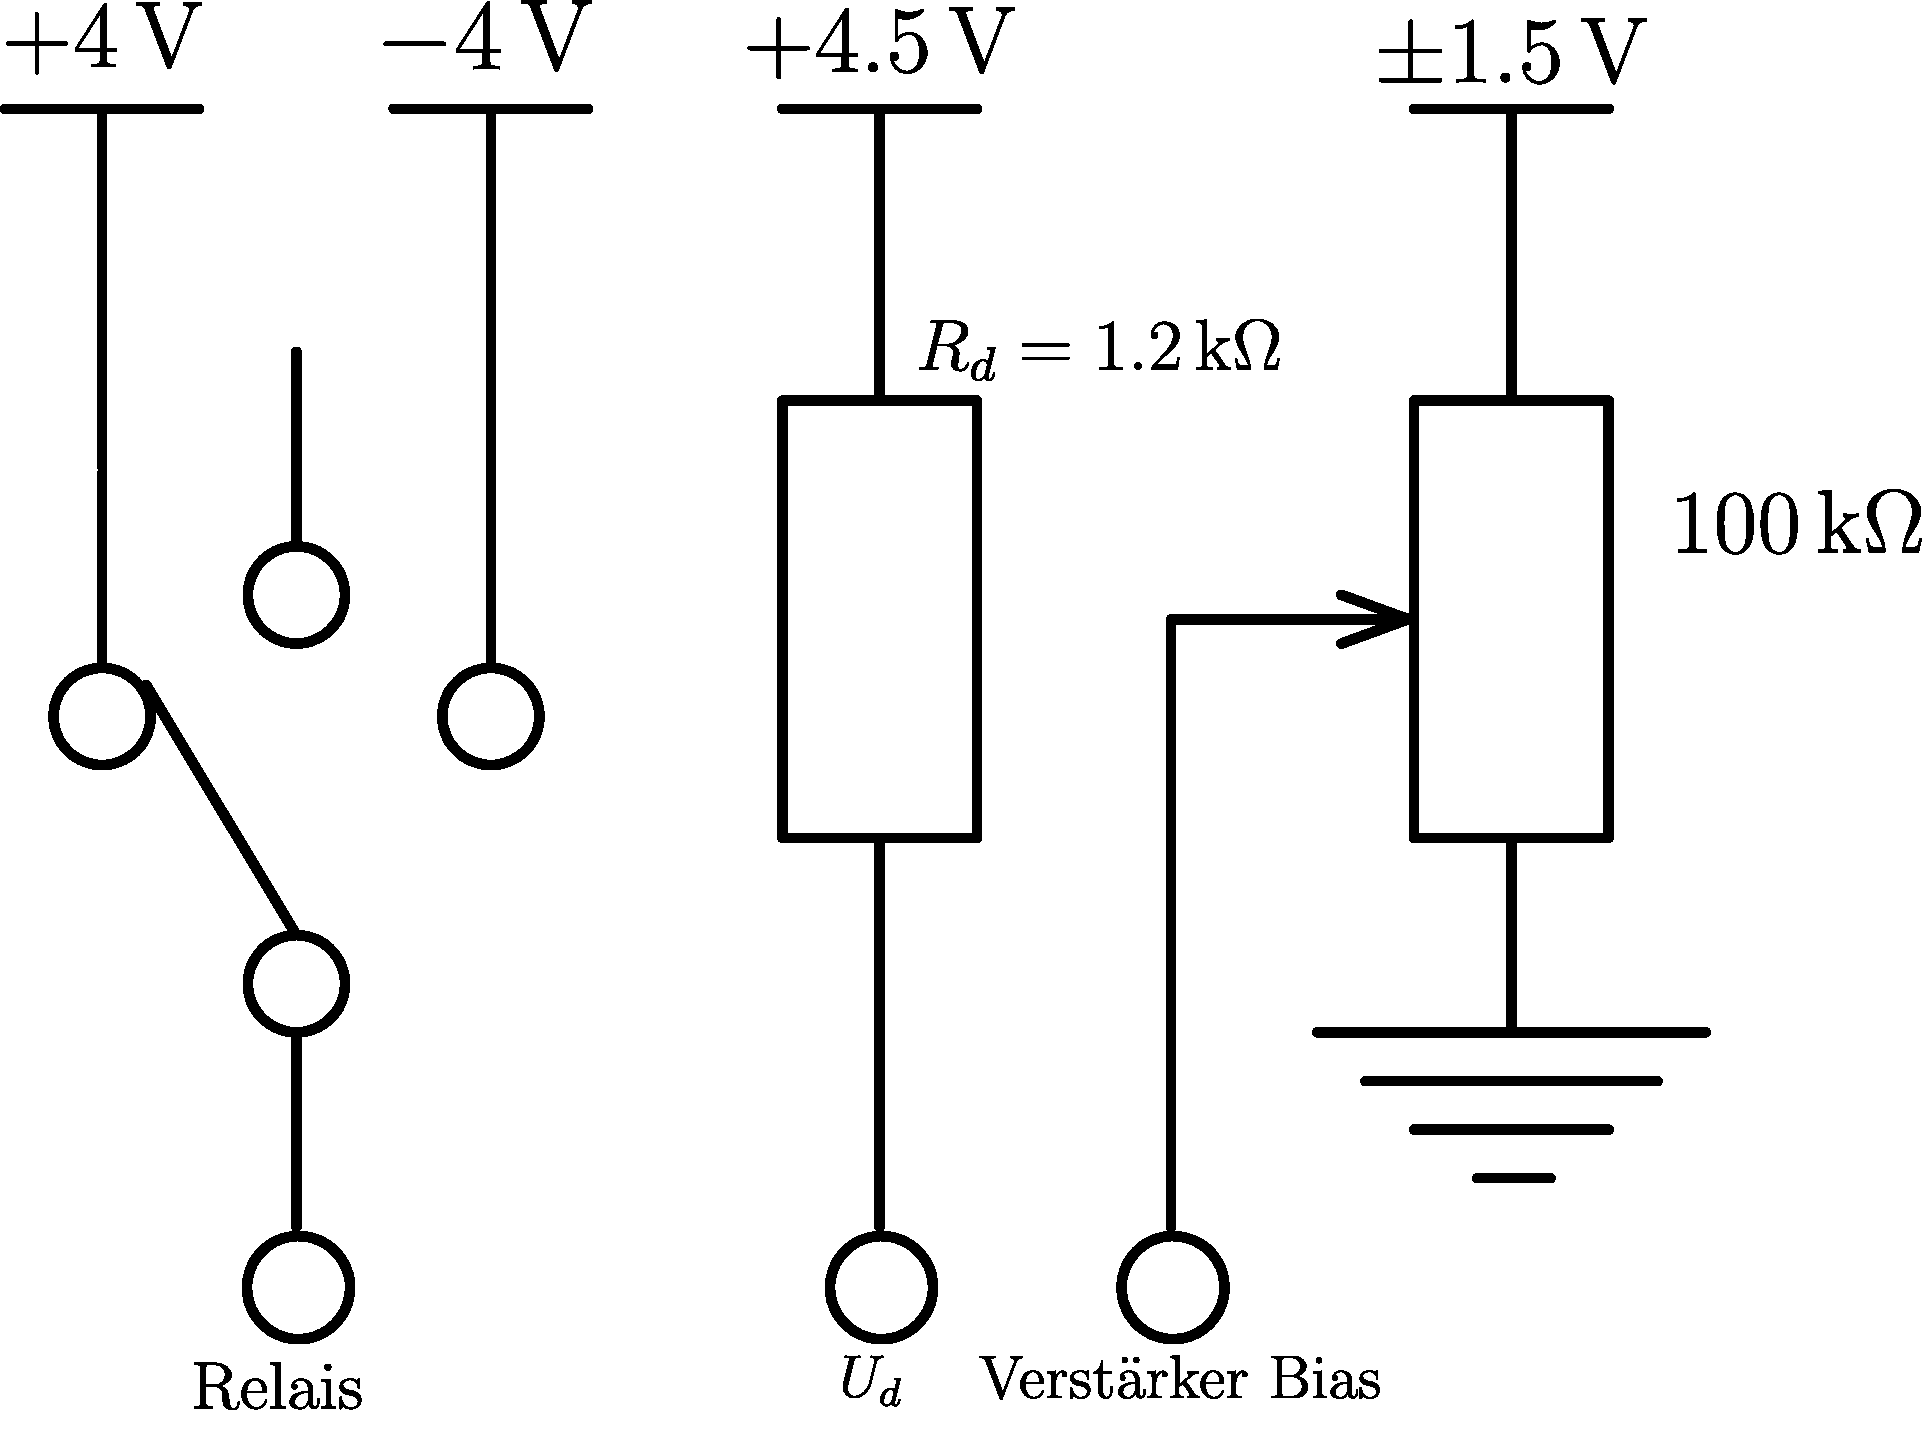
\includegraphics[width=0.5\textwidth]{./fig/Box.pdf}
\vspace{-0.5cm}
\caption{Schaltbild der warmen Elektronik mit einem dreistufigen Schalter zum schalten der Relais, dem Drainwiderstand des Verstärkers und einem Potentiometer um die Biasspannung am Gate des Verstärkers einzustellen.}
\label{fig:WarmeElektronik}
\end{center}
\end{figure}

Um die Handhabung der kalten Elektronik zu vereinfachen gibt es die in Abbildung \ref{fig:WarmeElektronik} gezeigte warme Elektronik.
Mit dem dreistufigen Kippschalter werden die Relais geschaltet.
Die Spannung $U_d$ und der Widerstand $R_d$ ist der Teil des Verstärkers welcher in Abbildung \ref{fig:Amp} außerhalb des Kryostaten ist.
Mit den $\SI{-1.5}{\volt}$ und dem $\SI{100}{\kilo\ohm}$ Potentiometer lässt sich die gewünschte Verstärker Biasspannung eingestellt.
Um das Rauschen zu minimieren und um Rückkopplung über die Spannungsquelle zu vermeiden wird die Drainspannung und die Verstärker Biasspannung mit unabhängigen Batterien versorgt.
Die Spannungen zum Schalten der Relais werden mittels Generator aufgebracht.
Im Warmen befindet sich außerdem ein Oszilloskop mit welchem das in Abbildung \ref{fig:Ausleseelektronik} dargestellte Ausgangssignal aufgenommen wird.
Und ein Signalgenerator mit welchem ein künstliches Signal einer bestimmten Frequenz erzeugt werden kann um die Verstärkung zu bestimmen.
Die Detektor Biasspannung ist für die Funktionsweise der Elektronik unbedeutend und wurde daher auf $\SI{0}{\volt}$ gesetzt.
In Abbildung \ref{fig:ElektronikBilder} sind Bilder der kalten Elektronik (oben Vorder- und Rückansicht) sowie der warmen Elektronik (unten) gezeigt.

Die Kühlung der kalten Elektronik findet mit flüssigem Stickstoff statt.
Dabei wird auf eine aufwendige Temperaturregelung verzichtet weshalb nur das Verhalten bei Raumtemperatur und flüssig Stickstoff Temperatur untersucht wird.
Schließlich befindet sich die kalte Elektronik in einem Faraday-Käfig um sie gegenüber elektromagnetischer Strahlung abzuschirmen.
Allerdings kann elektromagnetische Strahlung trotzdem über die langen Kabel zur Versorgung der Biasspannung und Drainspannung in die Elektronik gelangen.

Um den Aufbau so authentisch wie möglich zu gestalten in der kalten Elektronik ein \textit{dummy detector} eingebaut.
Dieser entspricht einer Kapazität zu Ground der selben Größe wie die Detektorkapazität $C_d$.

Die Daten der kalten Elektronik werden für verschiedenen handelsübliche HEMTs aufgenommen.

\begin{figure}[!t]
\begin{center}
\includegraphics[width=\textwidth]{./fig/ElektronikBilder.pdf}
\vspace{-0.5cm}
\caption{Bilder der warmen und kalten Elektronik.
Oben rechts: Rückseite der kalten Elektronik. Oben link: Vorderseite der kalten Elektronik.
Unten: Warme Elektronik im Gehäuse.}
\label{fig:ElektronikBilder}
\end{center}
\end{figure}


    \chapter{Auswertung der aufgenommenen Daten}
    Eine Prototyp Verstärkerelektronik nach dem in Kapitel \ref{sec:Elektronik} dargestellten Konzept wurde angefertigt und ist in Abbildung \ref{fig:ElektronikBilder} zu sehen.
In diesem Kapitel gehe ich auf die damit aufgenommenen Daten ein.

Im Vorfeld muss allerdings erwähnt werden, dass die Auswahl der verwendeten handelsüblichen HEMTs alle unter einem enorm großen Leckstrom leiden.
Die Datenblätter geben Ströme in der Größenordnung von $\SI{1}{} \-- \SI{10}{\micro\ampere}$ bei Raumtemperatur an \cite{ATF-54143, ATF-33143, ATF-34143}.
Das heißt bei geöffneten Relais entladen sich die Kondensatoren zu schnell sodass der Verstärker aus seinem Arbeitspunkt heraus driftet.
Grob überschlagen ergibt sich für die Zeitkonstante der Kondensatorentladung
\begin{equation}
\tau = RC =  \frac{U_{Bias}}{I_{Leck}}C  = \frac{\SI{100}{\milli\volt}\SI{100}{\pico\farad}}{\SI{1}{\micro\ampere}} = \SI{10}{\micro\second}.
\end{equation}
Daher werden die Messungen bei Raumtemperatur mit geschlossenen Relais durchgeführt.
Mit kleiner werdenden Temperaturen nimmt der Leckstrom allerdings ab sodass es bei flüssig Stickstoff Temperaturen möglich war den HEMT ATF-54143 bei offenen Relais zu operieren.
Sind die Relais der kalten Elektronik geschlossen muss insbesondere berücksichtigt werden, dass thermisches Rauschen der Widerstände hinzu kommt und dass die Kombination aus der Koppelkapazität $C_c$ und Biaswiderstand $R_b$ einen Hochpass mit der Grenzfrequenz $f_{-3\,\mathrm{db}}=1/2\pi R_bC_c=\SI{5.9}{\hertz}$ darstellen.
Durch größere Wahl des Biaswiderstand könnten beide Effekte weiter minimiert werden.


    \section{Temperatur- und Frequenzabhängigkeit der Verstärkung}\label{sec:AuswertungAmp}
    Um die Temperaturabhängigkeit und die Frequenzabhängigkeit der Verstärkung zu bestimmen wird ein Signalgenerator an der kalte Elektronik angeschlossen wo im Normalfall der Detektor angeschlossen wird.
Mit dem Signalgenerator können Sinussignale verschiedener Frequenzen erzeugt werden.
Das vom Signalgenerator erzeugte Eingangssignal sowie das Ausgangssignal des Verstärkers werden mit dem Oszilloskop aufgenommen.
Die Aufgenommenen Datenspuren werden geglättet um bursts des Signalgenerator zu entfernen.
Danach wird aus dem Verhältnis der Amplituden von Ausgangs- und Eingangssignal die Verstärkung bei gegebener Frequenz bestimmt.

\begin{minipage}[!c]{\textwidth}


\begin{minipage}[c]{\textwidth}
\begin{minipage}[c]{0.5\textwidth}
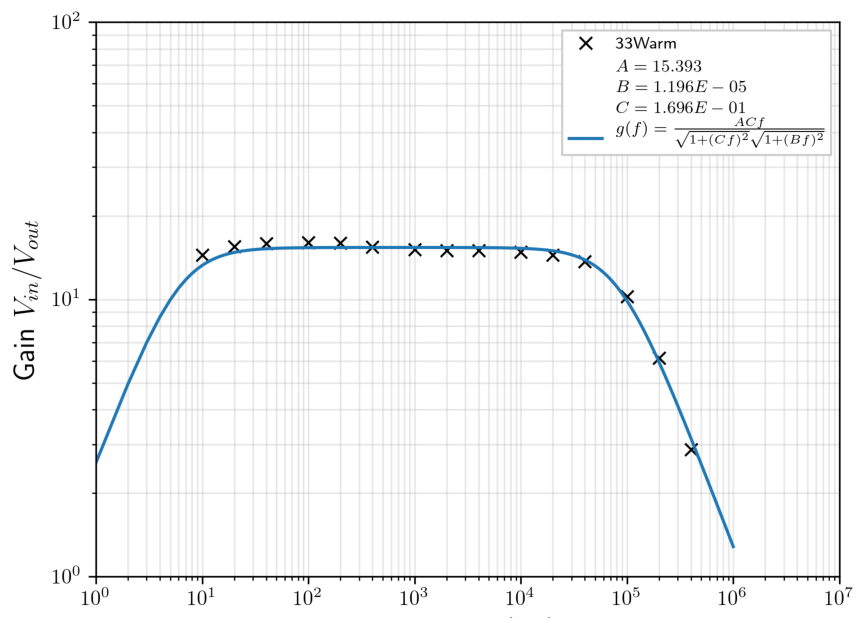
\includegraphics[width=\textwidth]{./fig/Gain/G33Warm.pdf}
\end{minipage}
\begin{minipage}[c]{0.5\textwidth}
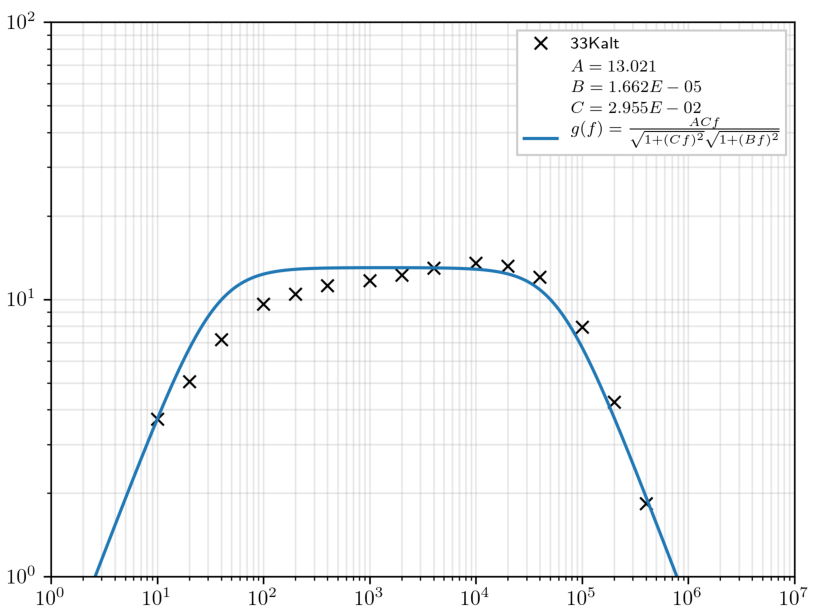
\includegraphics[width=\textwidth]{./fig/Gain/G33Cold.pdf}
\end{minipage}
\vspace{-0.45cm}
\captionof{subfigure}{Verstärkung der kalten Elektronik unter Verwendung des HEMTs ATF-33143\cite{ATF-33143}. Links: Verstärkung bei Raumtemperatur ($\SI{291}{\kelvin}$) und einer Biasspannung von $\SI{-0.6}{\volt}$. Rechts: Verstärkung bei flüssig Stickstoff Temperatur ($\SI{77}{\kelvin}$) und einer Biasspannung von $\SI{-1}{\volt}$.}
\label{subfig:33}
\end{minipage}

\begin{minipage}[c]{\textwidth}

\begin{minipage}[c]{0.5\textwidth}
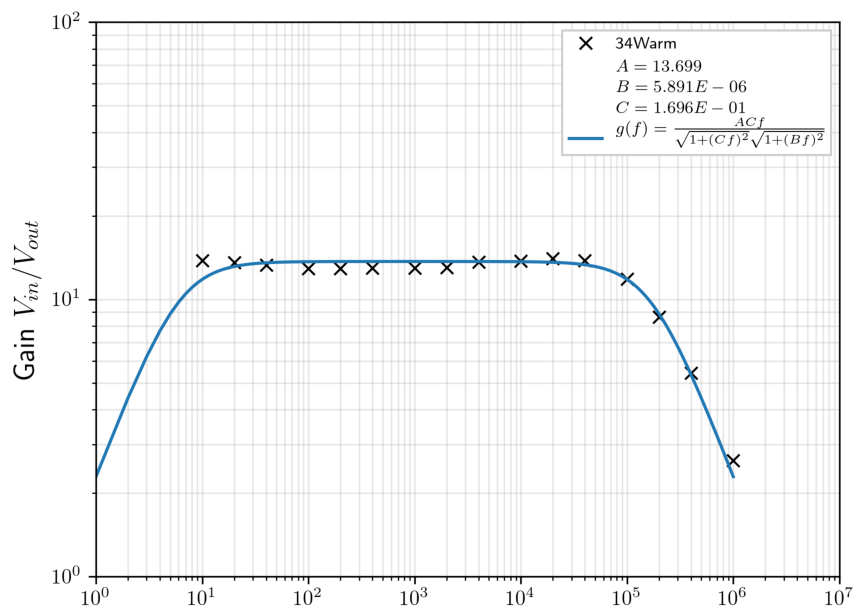
\includegraphics[width=\textwidth]{./fig/Gain/G34Warm.pdf}
\end{minipage}
\begin{minipage}[c]{0.5\textwidth}
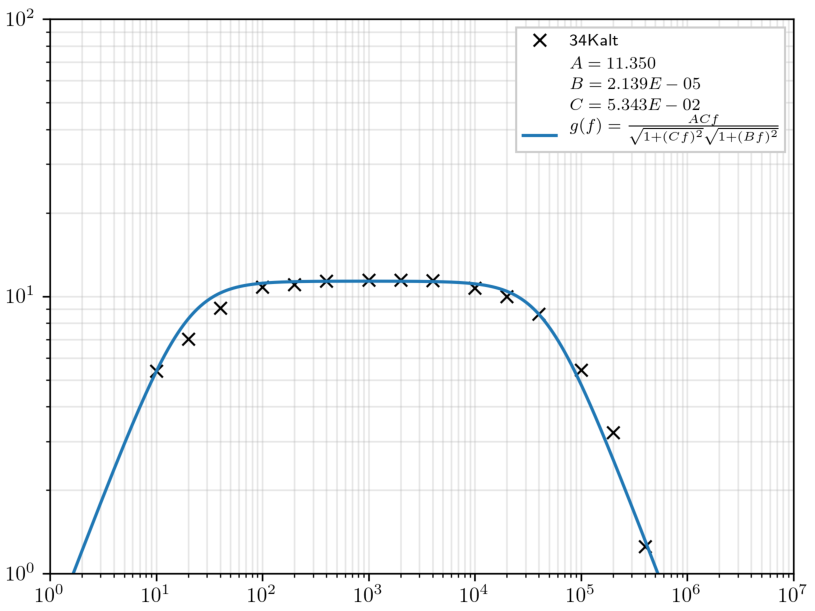
\includegraphics[width=\textwidth]{./fig/Gain/G34Cold.pdf}
\end{minipage}
\vspace{-0.45cm}
\captionof{subfigure}{Verstärkung der kalten Elektronik unter Verwendung des HEMTs ATF-54143\cite{ATF-34143}. Links: Verstärkung bei Raumtemperatur ($\SI{291}{\kelvin}$) und einer Biasspannung von $\SI{-0.74}{\volt}$. Rechts: Verstärkung bei flüssig Stickstoff Temperatur ($\SI{77}{\kelvin}$) und einer Biasspannung von $\SI{-0.94}{\volt}$.}
\label{subfig:34}
\end{minipage}

\begin{minipage}[c]{\textwidth}

\begin{minipage}[c]{0.5\textwidth}
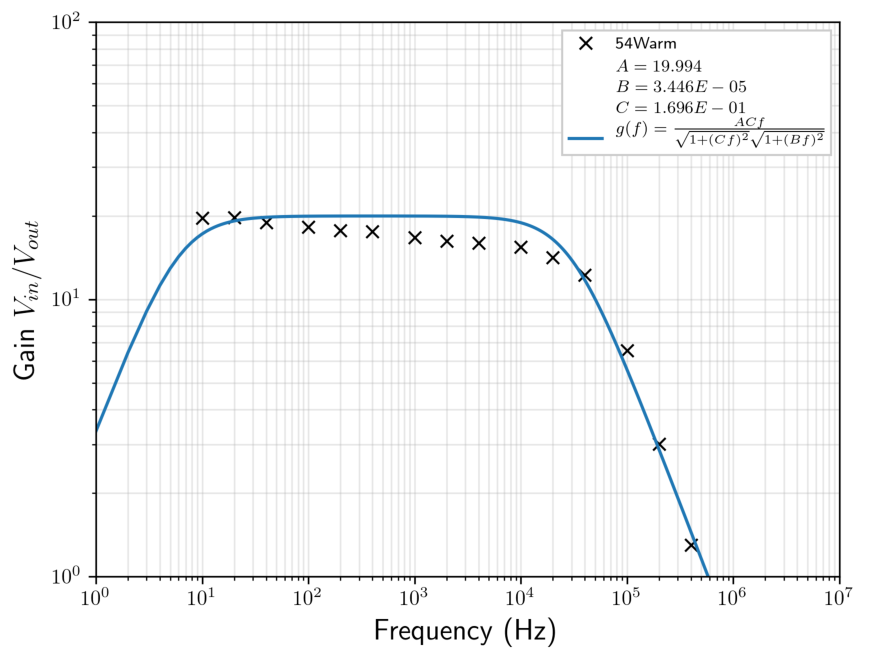
\includegraphics[width=\textwidth]{./fig/Gain/G54Warm.pdf}
\end{minipage}
\begin{minipage}[c]{0.5\textwidth}
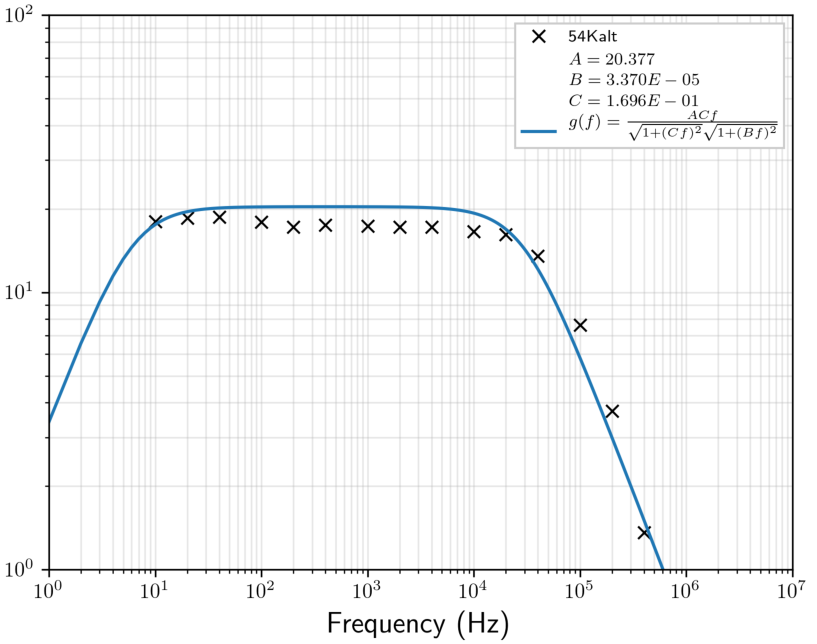
\includegraphics[width=\textwidth]{./fig/Gain/G54Cold.pdf}
\end{minipage}
\vspace{-0.45cm}
\captionof{subfigure}{Verstärkung der kalten Elektronik unter Verwendung des HEMTs ATF-54143\cite{ATF-54143}. Links: Verstärkung bei Raumtemperatur ($\SI{291}{\kelvin}$) und einer Biasspannung von $\SI{0.26}{\volt}$. Rechts: Verstärkung bei flüssig Stickstoff Temperatur ($\SI{77}{\kelvin}$) und einer Biasspannung von $\SI{0.38}{\volt}$.}
\vspace{-0.4cm}
\captionof{figure}{An die Daten (schwarz) ist die Übertragungsfunktion wie sie erwartet wird angepasst (blau). Die Konstante $A$ gibt die Verstärkung im konstanten Bereich an. Das inverse der Konstanten B die Grenzfrequenz des Tiefpass und das inverse der Konstanten C die Grenzfrequenz des Hochpass.}
\label{fig:Gain}
\end{minipage}
\end{minipage}

Die bei geschlossenem Relais aufgenommenen Daten sind in Abbildung \ref{fig:Gain} schwarz dargestellt.
An die Daten wurde die aus der Theorie erwartete Übertragungsfunktion angepasst (blau).
Diese setzt sich zusammen aus dem Hochpass welcher von der Kapazität $C_c$ und dem Widerstand $R_b$ gebildet wird mit der Grenzfrequenz $f^H_{-3\,\mathrm{db}} = \SI{5.9}{\hertz}$.
Und dem Tiefpass am Ausgang des Verstärkers aus $C_o$ und $R_o$ mit der Grenzfrequenz $f^T_{-3\,\mathrm{db}} = \SI{133}{\kilo\hertz}$.
\begin{equation}
U_a = U_e \frac{V_Uf}{\sqrt{1+(f/f^H_{-3\,\mathrm{db}})^2}\sqrt{1+(f/f^T_{-3\,\mathrm{db}})^2}}
\end{equation}

Zu sehen ist, dass die aus den Daten ermittelte Grenzfrequenz des Tiefpass in allen Fällen ungefähr einen Faktor $10$ kleiner ist als die erwartete.
Dies könnte auf die in der Theorie nicht berücksichtige Kapazität der Kabel liegen.
Um diesem Effekt entgegen zu wirken kann der Widerstand $R_o$ kleiner gewählt werden.

Der Effekt des Hochpasses ist nicht zu sehen da die aufgenommenen Daten nur bis zu einer minimalen Frequenz von $\SI{10}{\hertz}$ gehen.
Daher wurde für die aus der Theorie vorhergesagte Grenzfrequenz verwendet.
Ausgenommen davon sind die beiden HEMTs ATF-34143 und ATF-33143 welche beide im Kalten eine deutlich höhere Grenzfrequenz des Tiefpass aufweisen.

\begin{figure}[!b]
\begin{center}
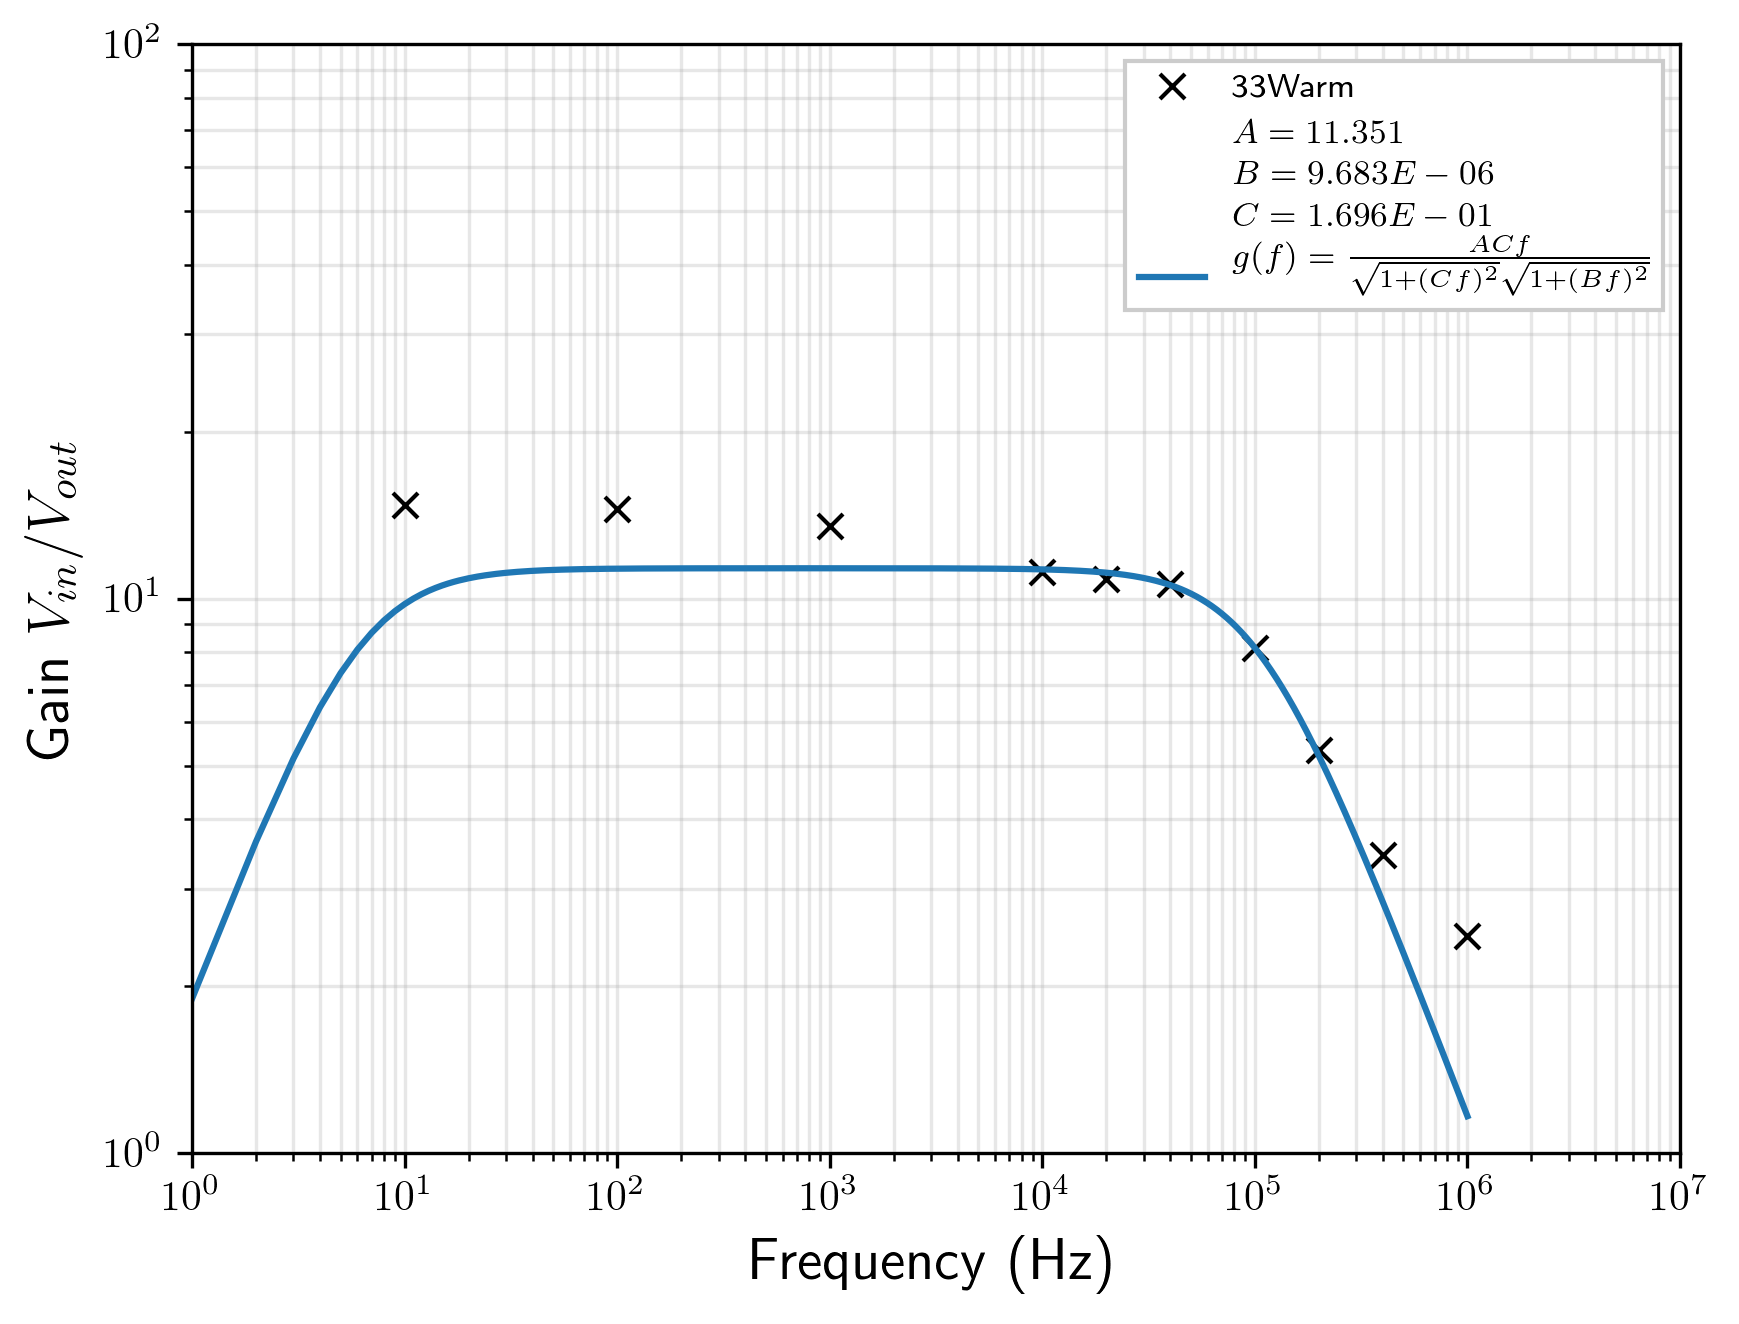
\includegraphics[width=0.65\textwidth]{./fig/Gain/G33WarmMarch21.png}
\vspace{-0.5cm}
\caption{Verstärkung des HEMTs ATF-33143 bei geschlossenem Relais, einem Drainwiderstand von $R_d = \SI{192}{\Omega}$ und einer Biasspanung von $\SI{-0.65}{\volt}$.}
\label{fig:33WarmGain100}
\end{center}
\end{figure}

Die Verstärkung aller drei HEMTs liegt in der Größenordnung von $10$ und ändern sich nur minimal mit der Temperatur.
Die aus der Theorie erwartete Verstärkung gegeben durch $-g_m R_d$ liegt allerdings deutlich höher bei $200\-- 400$ je nach HEMT.
Dies könnte zum einen daran liegen, dass die HEMTs am absoluten Rand ihres Ausgangskennlinienfeldes betrieben werden, d.h. mit deutlich weniger Strom als sie konzipiert sind.
Um weiter in die Mitte des Kennlinienfeldes zu gelangen muss der Drainwiderstand $R_d$ herabgesetzt werden.
Die Abbildung \ref{fig:33WarmGain100} zeigt die Verstärkung bei einem Drainwiderstand von $R_d=\SI{192}{\Omega}$ zu sehen ist, dass die Verstärkung beinah unverändert in der Größenordnung von $10$ bleibt die aus der Theorie erwartete Verstärkung allerdings auf $20 \-- 40$ runter geht.
Außerdem geht die verbrauchte Leistung hoch auf $\sim\SI{10}{\milli\watt}$.

Ein zweiter Grund könnte der Frequenzbereich sein indem die HEMTs verwendet werden.
Eigentlich sind handelsübliche HEMTs für den hochfrequenten Bereich von $\SI{500}{\mega\hertz}\--\SI{10}{\giga\hertz}$ konzipiert.
Daher haben sie auch sehr kleine Gate-Drain und Gate-Source Kapazitäten.
Die CRNS/LPN HEMTs dagegen sind speziell für den niederfrequenten Bereich und niedrigen Leistungsverbrauch ausgelegt.
Daher kann mit diesen eine deutlich höhere Verstärkung erreicht werden \cite{Phipps:2016mwv}.
Da diese zusätzlich über deutlich größere Eingangskapazitäten verfügen kann nicht länger der in Abschnitt \ref{sec:Amp} beschriebene Miller-Effekt vernachlässigt werden.
In diesem Fall kann statt einem Common-Source Verstärker zum Beispiel eine Kaskodenschaltung verwendet werden \cite{Gray}.

In Abbildung \ref{fig:54RClosed} ist die Verstärkung des HEMTS ATF-54143 bei offenem Relais gezeigt.
Dieser ist der einzige HEMT dessen Leckstrom mit $\SI{0.1}{\pico\ampere}$ klein genug ist bei flüssig Stickstoff Temperaturen sodass die Biasspannung über einen längeren Zeitraum gehalten wird.
Der Effekt des Hochpass entfällt und die Übertragungsfunktion wird zu
\begin{equation}
U_a = U_e \frac{V_U}{\sqrt{1+(f/f^T_{-3\,\mathrm{db}})^2}}.
\end{equation}

\begin{figure}[!t]
\begin{center}
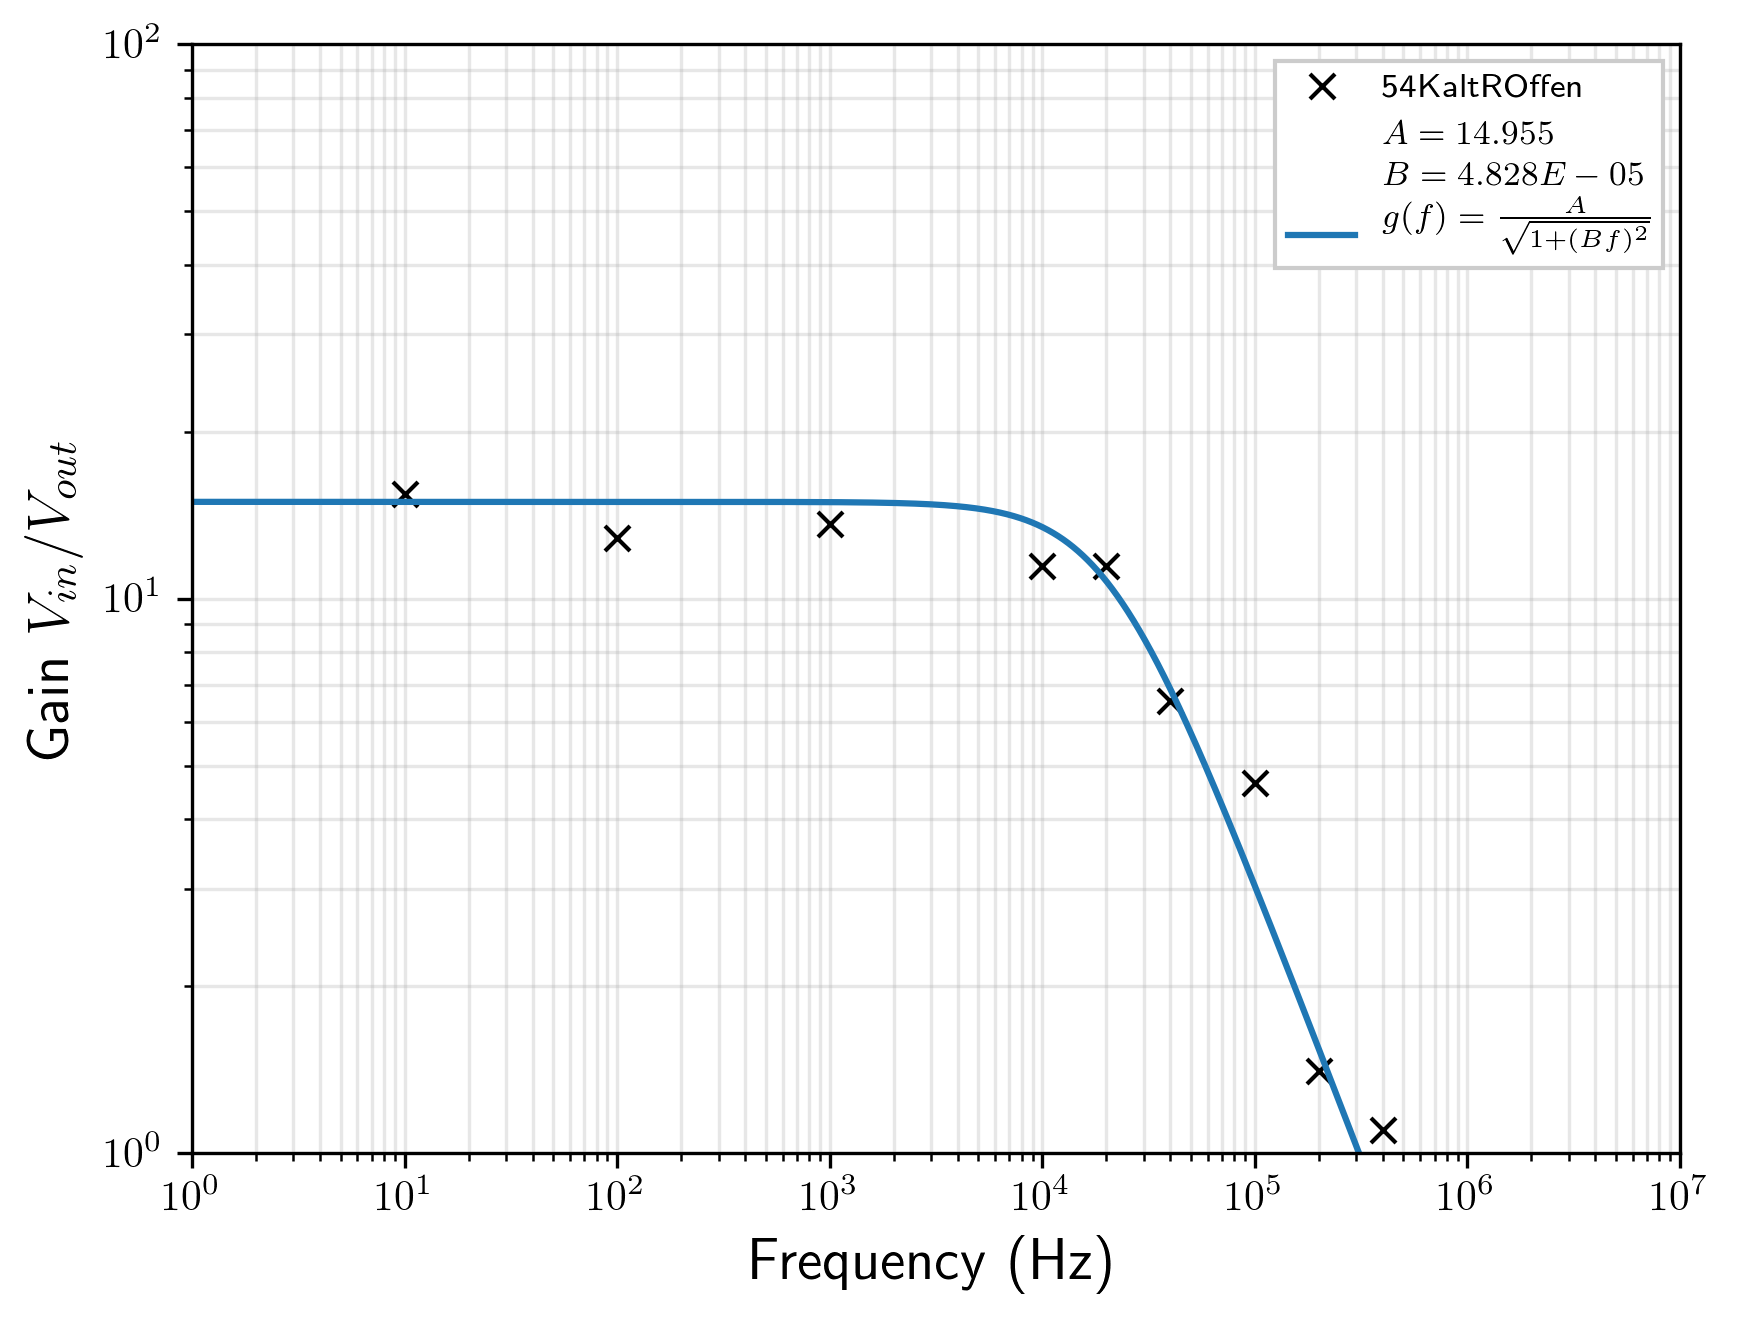
\includegraphics[width=0.65\textwidth]{./fig/Gain/G54ColdROpen.png}
\vspace{-0.5cm}
\caption{Verstärkung des HEMTs  ATF-54143 bei offenem Relais und einer Biasspannung von $\SI{0.371}{\volt}$.}
\label{fig:54RClosed}
\end{center}
\end{figure}




    \section{Vergleich der Rauschspektren bei verschiedenen Temperaturen}
    Zur Bestimmung der Rauschspektren wurden jeweils $16$ Datenspuren ohne angelegtes Signal mit einer Sampelrate von $f_s = \SI{100}{\kilo\hertz}$ aufgenommen.
Das Heißt die Nyquist-Frequenz, also die maximale auflösbare Frequenz, liegt bei $f_{Nq}=\SI{50}{\kilo\hertz}$.
Damit ist der interessante Teil des Spektrum abgedeckt.
Jenseits der $\SI{50}{\kilo\hertz}$ kommt dann der Effekt des Tiefpass zu tragen.
Für jede der Datenspuren wird die einseitige spektrale Leistungsdichte $J_{ss}(f_n)$ gemäß
\begin{equation}
\stackrel{\sim}{J}_{ss}(f_n) = 2 \frac{1}{N f_s}\left|\sum_i g(t_i)F(t_i)e^{-i\omega_n t_i}\right|^2
\end{equation}

\begin{minipage}[!c]{\textwidth}

\begin{minipage}[c]{\textwidth}
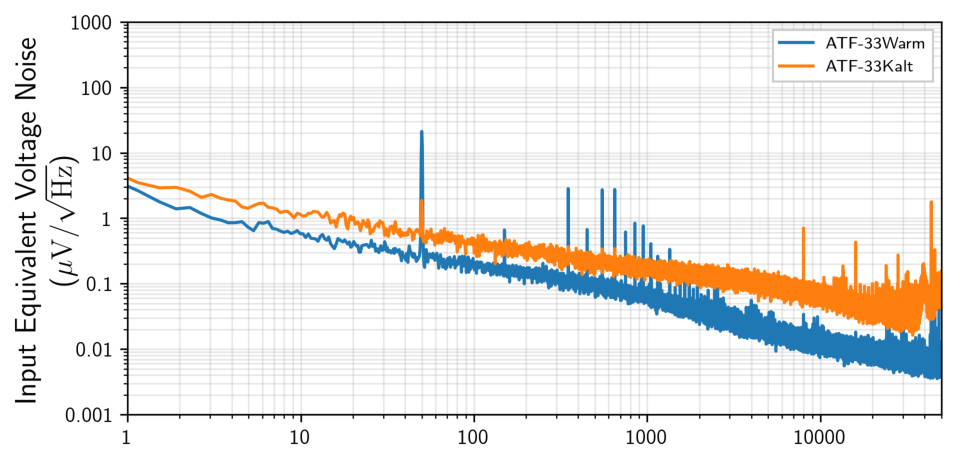
\includegraphics[width=\textwidth]{./fig/Rauschen/F33Warm.pdf}
\vspace{-0.45cm}
\captionof{subfigure}{Rauschen des HEMT ATF-33143}
\label{subfig:33}
\end{minipage}

\begin{minipage}[c]{\textwidth}
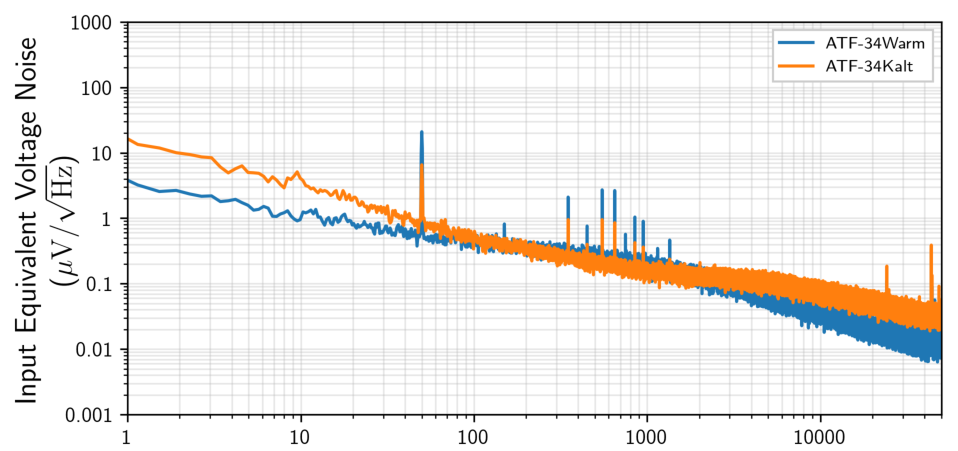
\includegraphics[width=\textwidth]{./fig/Rauschen/F34Warm.pdf}
\vspace{-0.45cm}
\captionof{subfigure}{Rauschen des HEMT ATF-34143}
\label{subfig:33}
\end{minipage}

\begin{minipage}[c]{\textwidth}
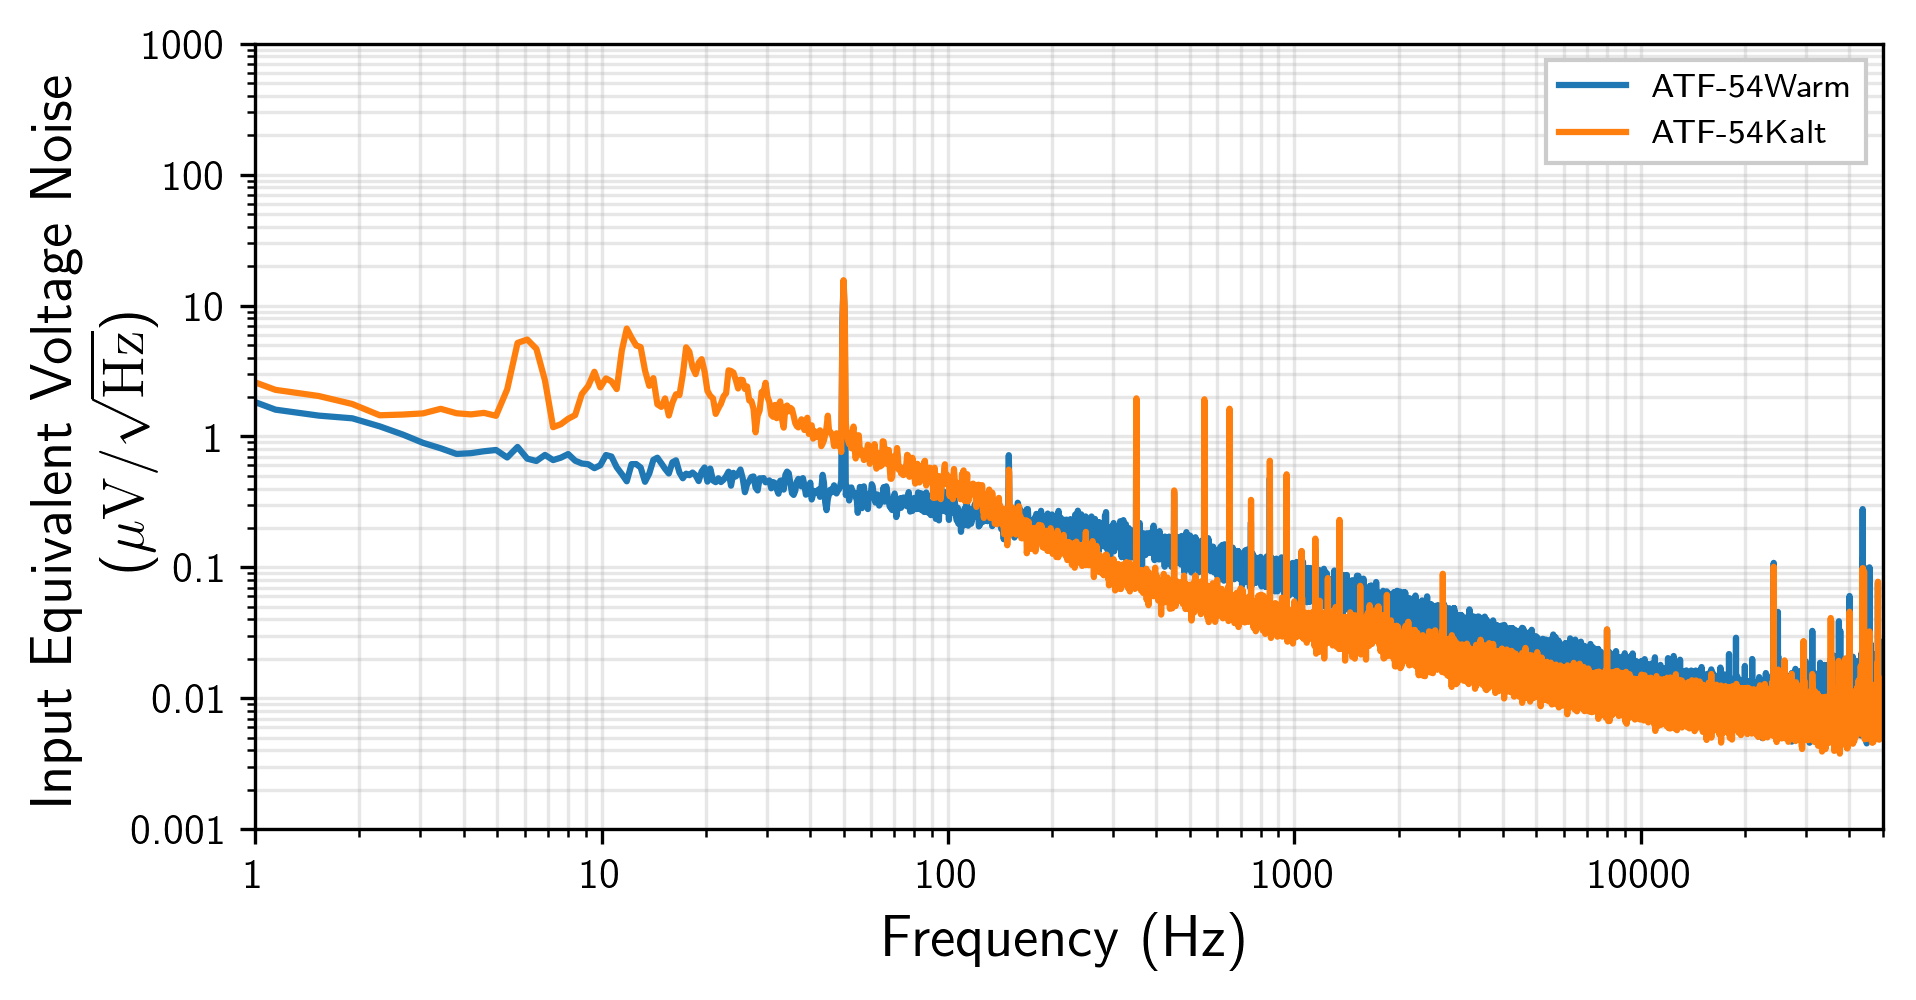
\includegraphics[width=\textwidth]{./fig/Rauschen/F54Warm.png}
\vspace{-0.45cm}
\captionof{subfigure}{Rauschen des HEMT ATF-54143}
\label{subfig:33}
\end{minipage}

\vspace{-0.4cm}
\captionof{figure}{Eingangsseitige Leistungsdichtespektren verschiedener HEMTs, bei geschlossenem Relais.
Bei Raumtemperatur (Warm) $\SI{291}{\kelvin}$ und bei flüssig Stickstoff Temperatur (Kalt) $\SI{77}{\kelvin}$.
Die gleiche Biasspannungen wie bei der Bestimmung der Verstärkung wurden verwendet.}
\label{fig:RauschenOpen}
\end{minipage}

mit der Fensterfunktion $F(t_i)$ bestimmt und über alle Spuren gemittelt.
Das auf diese weise erhaltene ausgangsseitige Leistungsspektrum wird durch das Quadrat der in Abschnitt \ref{sec:AuswertungAmp} erhaltenen Übertragungsfunktionen geteilt um das eingangs seitige Rauschen zu erhalten.

In Abbildung  ist $\sqrt{J_{ss}(f_n)}$ der verschiedenen HEMTs und Temperaturen dargestellt.
Alle Spektren weisen den erwarteten $\SI{50}{\hertz}$ Peak und seine harmonischen auf.
Mit der Verwendung von Batterien konnte dieser allerdings deutlich verringert werden.
Abgesehen davon treten im niederfrequenten Bereich sonst keine dominanten Peaks aus.
Erst im höherfrequenten Bereich jenseits der $\SI{10}{\kilo\hertz}$ treten vereinzelte Peaks auf welche vermutlich auf Umwelt Störeinflüsse zurückzuführen sind da sie nicht einheitlich bei allen Spektren auftreten.
Auffallend ist allerdings, dass für alle Spektren das Rauschen im niederfrequenten Bereich deutlich ansteigt bei flüssig Stickstoff Temperatur.
Eine mögliche Erklärung könnte sein, dass durch das sieden des Flüssigen Stockstoff Vibrationen entstehen welche in die Elektronik einkoppeln können.
Die gleichen Beobachtungen wurde auch in den Rauschspektren der EDELWEISS-III Ausleseelektronik von Axel Gullasch gemacht \cite{Gullasch2015}.
Da die Elektronik unmittelbar in den siedende Stickstoff eingetaucht wurde könnte dieser Effekt hier sogar noch größer sein.

Das beste Rauschspektrum ist in Abbildung \ref{fig:54RClosed} dargestellt und wurde wie erwartet bei offenem Relais erreicht, da das Rauschen durch die Biaswiderstände, Kabel und Spannungsquellen nicht mehr auftritt.
Im Vergleich mit dem Besten Rauschen der EDELWEISS-III Ausleselektronik \ref{fig:EDWIII} ist zu sehen, dass der HEMT basierte Verstärker ein deutlich geringeres Rauschen vor allem im niederfrequenten Bereich aufweist.
Hinzu kommt, dass der Auftretende $\SI{50}{\hertz}$ Peak und seine Harmonischen eine deutlich geringere Amplitude aufweisen.

\begin{figure}[!b]
\begin{center}
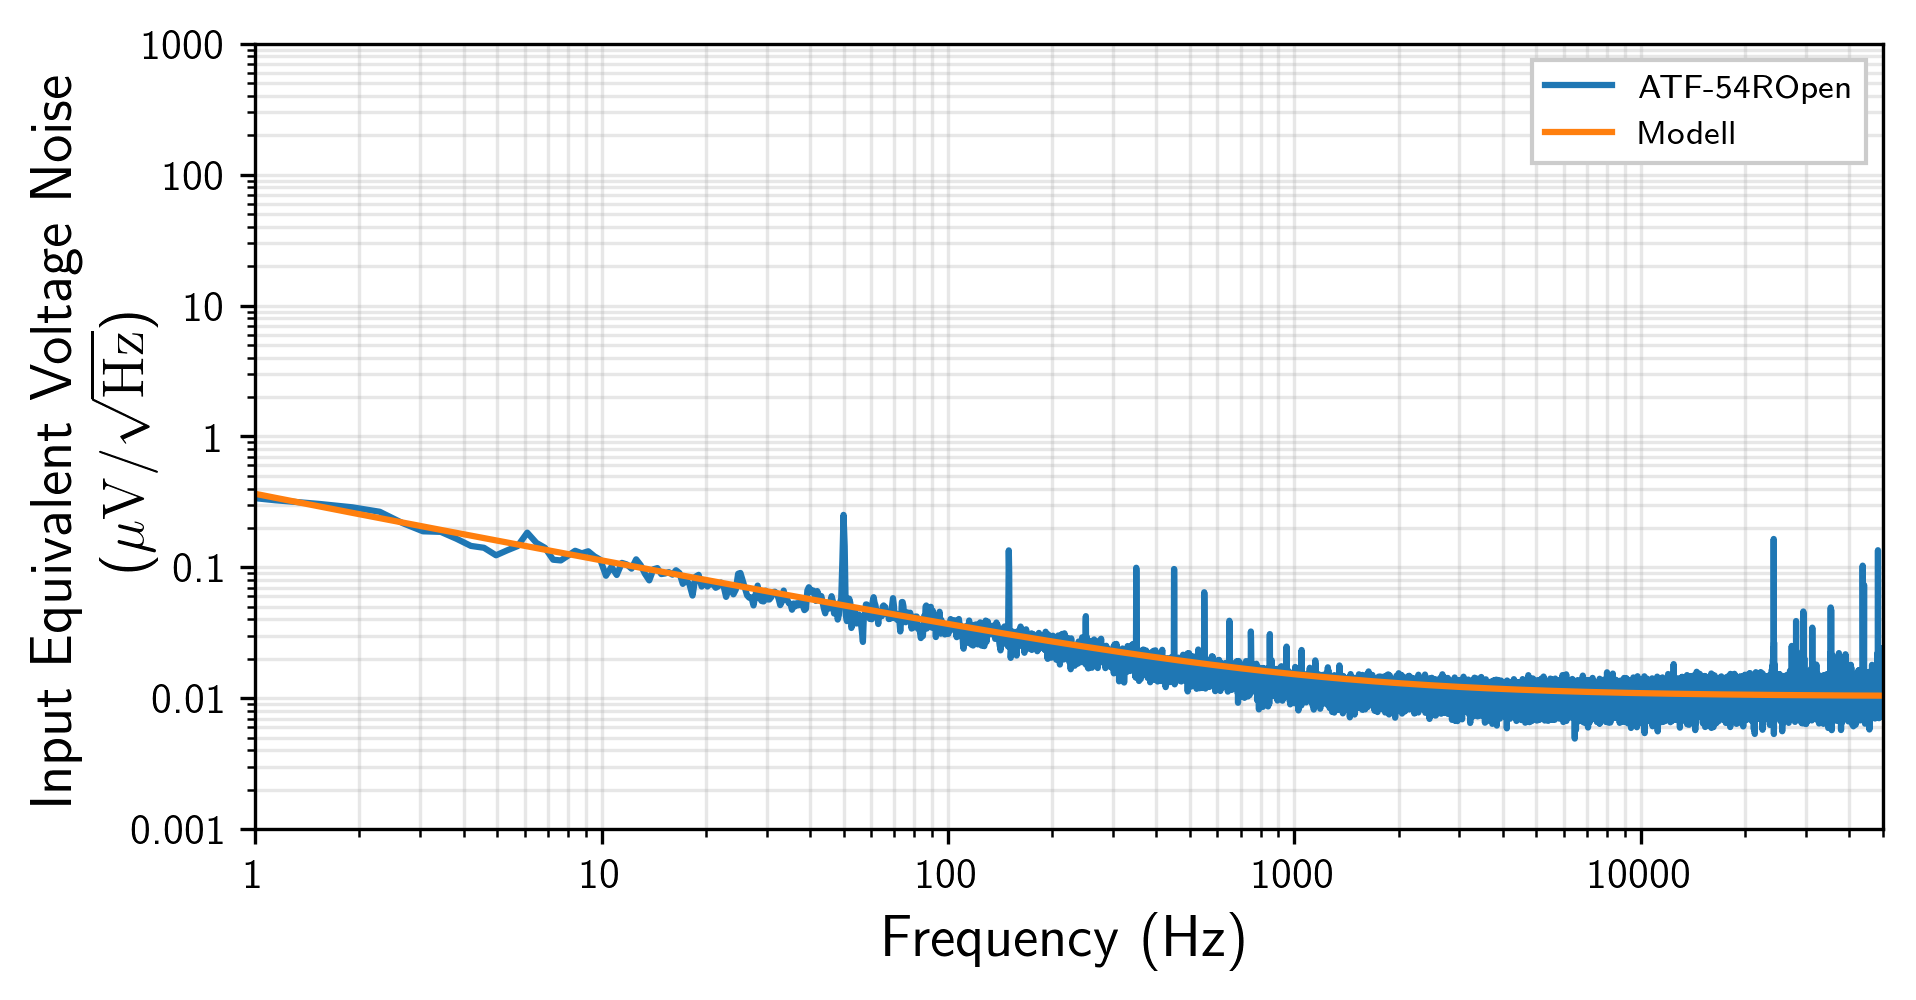
\includegraphics[width=\textwidth]{./fig/Rauschen/F54ROpen.png}
\vspace{-0.5cm}
\caption{Rauschen des HEMTs  ATF-54143 bei offenem Relais und einer Biasspannung von $\SI{0.371}{\volt}$.}
\label{fig:54ROpen}
\end{center}
\end{figure}

Das in Abschnitt \ref{sec:Rauschen} beschriebene Modell zur Beschreibung des Rauschen wurde an die gemessenen Daten Angepasst.
Da sich die gemessenen Daten sowohl aus dem Rauschen der Spannungsquelle $u_r$ und dem der Stromquelle $i_r$ zusammensetzen ist die Bestimmung des Rauschen der einzelnen quellen nicht möglich.
Für das gesamte Rauschen ergibt sich dann
\begin{equation}
u^2_{ges} = \frac{(\SI{8.3e-8}{})^2}{f^2} + \frac{(\SI{3.5e-7}{})^2}{f} + (\SI{1.0e-8}{})^2 \quad (\SI{}{\volt\squared\per\hertz}).
\end{equation}
Um das Rauschen der Quellen einzeln zu bestimmen muss zuerst der Eingang des Verstärkers geerdet werden dadurch verschwindet das Rauschen der Stromquelle und das der Spannungsquelle kann bestimmt werden.
Im Anschluss kann dann bei bekanntem rauschen der Spannungsquelle das der Stromquelle bestimmt werden.

Der Leckstrom wird aus dem Schortrauschen bestimmt.
Ein Vergleich des gemessenen $1/f^2$-Rauschen mit dem theoretisch erwarteten entsprechend Gl. \ref{eq:Rauschen} zeigt
\begin{equation}
\frac{a + 2eI_{Leck}}{4\pi^2C^2_{ges}} = (\SI{8.3e-8}{})^2.
\end{equation}
Mit der Annahme, dass der Parameter $a=0$ ist ergibt sich für den Leckstrom eine obere Abschätzung von
\begin{equation}
I_{Leck} = \SI{1.4}{\femto\ampere}.
\end{equation}

\begin{figure}[!b]
\begin{center}
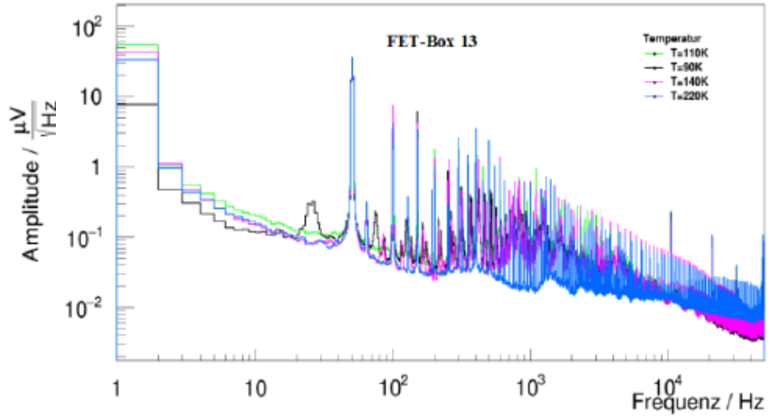
\includegraphics[width=\textwidth]{./fig/Rauschen/GullaschRauschen.pdf}
\vspace{-0.5cm}
\caption{Beste Leistungsdichtespektren der EDELWEISS-III Ausleseelektronik von Axel Gullasch \cite{Gullasch2015}.}
\label{fig:EDW}
\end{center}
\end{figure}
    \section{Bestimmen der Energieauflösung}
	\begin{figure}[!t]
\begin{center}
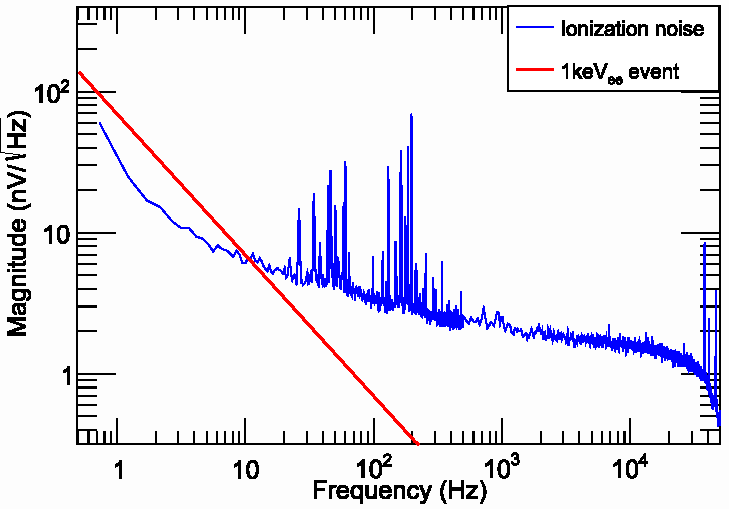
\includegraphics[width=\textwidth]{./fig/Rauschen/EDWIIIPerformance.pdf}
\vspace{-0.5cm}
\caption{Leistungsdichtespektren der EDELWEISS-III Ausleseelektronik \cite{EDWIII}.}
\label{fig:EDWIII}
\end{center}
\end{figure}

Eine Aussage über die Energieauflösung ist erst möglich wenn sowohl das Rauschen als auch die Form des Signals bekannt sind.
Für die Bestimmung der Energieauflösung ist es also notwendig einen Beispielsignal wie wir es erwarten würden zu bestimmen.
Wie in den Kapiteln \ref{sec:Entstehung} und \ref{sec:Elektronik} gezeigt erzeugt ein Event welches die Energie $E$ deponiert eine bestimmte Zahl Elektron-Loch-Paare $N_{eh}$ abhängig von einer Materialspezifischen mittleren Energie zur Erzeugung eines Elektron-Loch-Paars $\epsilon$.
Für den Strom der durch ein solches Event in der Elektronik induziert wird ergibt sich somit
\begin{equation}
I_{sig}(t) = e\frac{E}{\epsilon}(a-b)\delta (t).
\end{equation}
Durch die transformation in den Frequenzraum und Multiplikation mit der Eingangsimpedanz erhalten wir das Spektrum des Signals
\begin{equation}
s(f) = e\frac{E}{\epsilon}(a-b)\frac{1}{2\pi f C_{ges}}.
\end{equation}
Die Bestimmung der Energieauflößung mittels der Optimal Filtering Methode ist gegeben durch
\begin{equation}
\sigma^2_E = \left(\sum_{f_{min}}^{f_{max}}\frac{|s(f)|^2}{J_{ss}(f)}\Delta f\right)^{-1}
\label{eq:OptFilt}
\end{equation}
$f_{max}$ - $f_{min}$ ist die Bandbreite, $J_{ss}$ die Leistungsspektrumdichte für $f>0$ und $\Delta f$ der Abstand zwischen den gemessenen Frequenzen.
Aus dieser Gleichung lässt sich erkennen, dass die Verstärkung keinen Einfluss auf die Auflösung hat, da sowohl das signal $s(f)$ als auch das Rauschen $J_{ss}$ gleichermaßen verstärkt werden.
Die Verstärkung muss nur groß genug sein sodass das Rauschen der Nachfolgenden Elektronik keine Rolle spielt.
Auf diese Weise wurde für das in Abbildung \ref{fig:54ROpen} gezeigte Rauschen eine Energieauflöung von $\boldsymbol{\sigma_E = \frac{1}{a-b}\cdot 1.31\,\mathrm{keV}}$ berechnet unter der Annahme einer Detektorkapazität von $\SI{150}{\pico\farad}$.
Man sieht, dass die Auflösung proportional zum Prozentsatz des von den Ladungsträgern durchlaufenen Potentials $(a-b)$ ist.

In Abbildung \ref{fig:EDWIII} ist das Leistungsdichtespektrum der EDELWEISS-III Ausleseelektronik dargestellt zusammen mit einem $\SI{1}{\kilo\electronvolt}$ Beispielsignal.
Damit wurde eine Energieauflösung von $\SI{500}{\electronvolt}$ erreicht\cite{EDWIII} unter Verwendung eines $\SI{150}{\pico\farad}$ Detektor mit zusätzlich $\SI{100}{\pico\farad}$ Kapazität durch die Kabel und $\SI{50}{\pico\farad}$ Eingangskapazität des JFET.
Die beste von Axel Gullasch erreichte Energieauflößung mit der gleichen Elektronik ist $\SI{2.11}{\kilo\electronvolt}$ \cite{Gullasch2015}.
%TODO Detektorkapazität nicht bestimmt Gullasch
Mit CRNS/LPN HEMTs ist eine Energieauflösung von $\SI{91}{\electronvolt}$ mit einem $\SI{150}{\pico\farad}$ CDMS-Detektor gelungen \cite{Phipps2016}.


    
    \chapter{Ausblick}
    Ein Detektor mit Vakuum separierte Elektrode hat den Vorteil einer besseren Energieauflösung im Wärmekanal auf kosten eines abgeschwächten Signals im Ionisationskanal.
Um die Luke-Verstärkung zu überprüfen ist es notwendig das Ionisationssignal in beiden Kanälen auszulesen.
im Ionisationskanal sollen dazu Signale von $\gamma$-Quellen im $\SI{}{\kilo\electronvolt}$ Bereich sichtbar sein.
In dieser Arbeit wurde eine Verstärkerelektronik entwickelt um den Ionisationskanal auszulesen sie fungiert gleichzeitig als Impedanzwandler damit der Signalstrom nicht von den langen Kabeln und der Digitalisierung belastet wird.
Diese ist dazu ausgelegt ohne zusätzliche Heizung im Kryostaten bei $\SI{4}{\kelvin}$ zu operieren.
Dazu wurden handelsübliche HEMTs verwendet mit dem Vorteil der leichten Verfügbarkeit aber unter großen Leckströmen und großem niederfrequentem Rauschen leiden.
Die Elektronik wurde bei Raumtemperatur und flüssig Stickstofftemperatur getestet.
Bei Raumtemperatur ist der Leckstrom aller HEMTs zu groß um die Elektronik wie vorgesehen mit Vorgespannten Kondensatoren und offenem Relais zu operieren.
Mit abnehmender Temperatur nimmt allerdings auch der Leckstrom ab, sodass es möglich war einen HEMT über einen längeren Zeitraum bei offenem Relais zu operieren.
Mit allen HEMTs wurde eine Spannungsverstärkung in der Größenordnung von $\mathcal{O}(10)$ erreicht.
Das Rauschen ist etwa einen Faktor $10$ größer als das der EDELWEISS-III bei $\SI{4}{\kelvin}$ Elektronik\cite{EDWIII}.
Ein Teil des Rauschen kann durch den siedenden Stickstoff verursacht sein in welchen die Elektronik eingetaucht wurde.
Dafür spricht, dass das Rauschen im Kalten größer wurde.
Die selbe Beobachtung wurde auch schon in der Arbeit von Axel Gullasch\cite{Gullasch2015} gemacht.
Ein Leckstrom von $\SI{1,4}{\femto\ampere}$ wurde bestimmt.
Aus dem Leistungsdichtespektrum des Rauschen wurde mittels der optimal filtering Methode(siehe Abschnitt \ref{sec:OptFilt}) die Energieauflösung anhand des erwarteten Signalpuls zu $\frac{1}{a-b}\SI{1,31}{\kilo\electronvolt}$ bestimmt.
Um die Energieauflösung mit der EDELWEISS-III Elektronik von $\SI{500}{\electronvolt}$ zu vergleichen wurde auch eine $\SI{150}{\pico\farad}$ Detektorkapazität angenommen.
Die Elektronik sollte noch unter den Bedingungen wie sie im Experiment gegeben sind, $\SI{4}{\kelvin}$ und ein Richtiger Detektor, getestet werden.
Um die Schaltung noch weiter zu optimieren besteht die Möglichkeit CNRS/LPN HEMTs zu verwenden welche hervorragende Eigenschaften für unsren Anwendungsfall aufweisen. 

    % appendix for more or less interesting calculations

    % to make the appendix appear in ToC without number. \appendixname = 
    % Appendix or Anhang (depending on chosen language)
    %\input{./chap/appendix.tex} %\cleardoublepage



    % Bibliography
    \TheBibliography

    % BIBTEX
    % use if you want citations to appear even if they are not referenced to: 
    % \nocite{*} or maybe \nocite{Kon64,And59} for specific entries
    %\nocite{*}
    %\bibliographystyle{abbrv}
    
    \printbibliography \addcontentsline{toc}{chapter}{Literaturverzeichnis}
	\listoffigures %\addcontentsline{toc}{chapter}{Abbildungsverzeichnis}
	\chapter*{Abkürzungsverzeichnis}
	\addcontentsline{toc}{chapter}{Abkürzungsverzeichnis}
	\begin{acronym}
\acro{SM}{Standard Modell}
\acro{DM}{Dunkler Materie}
\acro{WIMP}{weakly interacting massive particle}
\acro{LDM}{light dark matter}
\acro{MOND}{Modified Newtonian dynamics}
\acro{PQ}{Peccei-Quinn}
\acro{SUSY}{Supersymmetrie}
\acro{CP}{Charge-Parity Symmetrie}
\acro{MMC}{metallic magnetic calorimeter}
\acro{RKKY}{Ruderman-Kittle-Kasuya-Yoshida}
\acro{SQUID}{super quantum interference device}
\acro{LUX}{Large Underground Xenon experiment}
\acro{XENON}{Ein flüssig Xenon Experiment}
\acro{SuperCDMS}{Cryogenic Dark Matter Search}
\acro{EDELWEISS}{Expérience pour DEtecter Les WIMPs En Site Souterrain}
\acro{HEMT}{High electron mobility transistor}
\acro{JFET}{junction field-effect transistor}
\acro{MOSFET}{metal-oxide-semiconductor field-effect transistor}
\acro{CNRS}{Centre for Nanosciences and Nanotechnology}
\end{acronym}
    %\listoftables
    \Appendix
    \chapter{\appendixname} %\addcontentsline{toc}{chapter}{\appendixname}
    \section{Optimal Filtering}\label{sec:OpFiltering}
    In diesem Abschnitt werden ein paar grundlegende Erkenntnisse der optimal filtering Methode dargestellt.
Die Darstellung orientiert sich anhand \cite{Golwala2000, Enss2005}.

\subsection{Diskrete Fouriertransformation}
In der Realität können Signale nicht kontinuierlich abgetastet werden und nur über einen begrenzten Zeitraum aufgenommen.
Die Fouriertransformation muss daher für den diskreten Fall angepasst werden zu
\begin{align*}
\widetilde{v}_n &= \frac{1}{N}\sum_{k=-N/2}^{N/2} v_k e^{-i2\pi f_n t_k} \\
v_k &= \sum_n \widetilde{v}_{n=n=-N/2}^{N/2} e^{i2\pi f_n t_k}
\end{align*}
der Spurlänge $N=Tf_s$, welche sich aus der Spurdauer $T$ und Sample Rate $f_s$ ergibt, Zeitpunkten $t_k = k\Delta T = k/f_s$ und Frequenzen $f_n = n/T$.
Aufgrund der endliche Spurdauer kommt es zu Frequenzbins der Breite $f_{n+1}-f_n=1/T$.
Aufgrund der endlichen Abtastrate wird die Bandbreite durch die Nyquest-Frequenz $f_{Nq}=f_{N/2}=N/2T=f_s/2$, welche der halben Abtastrate entspricht, begrenzt.

\subsection{Rauschen}
Die Fluktuationen der Spannung werden als gaussverteilt angenommen mit der Varianz $\langle\left[v(t)\right]^2\rangle$.
Die Varianz beschreibt das Rauschen allerdings nicht vollständig, da Korrelationen des Signals nicht berücksichtigt werden.
Korrelationen treten auf, da eine Fluktuation der Spannung mit einer bestimmte Zeitkonstante $\tau$ abfällt und daher $v(t)$ Informationen über $v(t+\tau)$ enthält.
Die Autokorrelationsfunktion $R(\tau)$ berücksichtigt die Korrelation
\begin{align*}
R(\tau) &= \langle v(t)v(t+\tau)\rangle \\
&= \lim_{T\rightarrow \infty}\frac{1}{T}[v\otimes v](\tau) \\
&= \lim_{T\rightarrow \infty}\frac{1}{T}\int_{-T/2}^{T/2}\,dt\, v(t)v(t+\tau)
\end{align*}
$\otimes$ steht hier für die Kreuzkorrelation.
Äquivalent kann das Rauschen im Frequenzraum dargestellt werden.
Dies hat den Vorteil, dass für lineare Systeme das Rauschen unterschiedlicher Frequenzen nicht korreliert ist.
Die spektrale Leistungsdichte $J(f)$ ist gegeben durch die Fouriertransformation der Autokorrelationsfunktion und hat die Einheit $\SI{}{\volt^2\per\hertz}$
\begin{equation}
J(f) = \lim_{T\rightarrow \infty}\int_{-T}^{T}\, dt\, R(t) e^{-jwt}.
\end{equation}
Entsprechend gilt 
\begin{align*}
R(t) &= \lim_{T\rightarrow \infty}\int_{-T}^{T}\,df\, J(f) e^{jwt} \\
\Rightarrow \langle\left[v(t)\right]^2\rangle &= R(0) = \int_{-\infty}^{\infty}\,df\, J(f).
\end{align*}
Das Integral der spektralen Leistungsdichte gibt also die Varianz des Rauschen. 

Die spektrale Leistungsdichte wird in der Regel nicht aus der Autokorrelationsfunktion bestimmt sondern direkt aus Fourier transformierten Spuren ohne Signale.
Es gilt
\begin{align*}
J(f) &= \lim_{T\rightarrow \infty}\int_{-T}^{T}\,dt\, R(t) e^{-jwt} \\
&= \lim_{T\rightarrow \infty}\int_{-T}^{T}\,dt\,e^{-jwt}\lim_{T\rightarrow \infty}\frac{1}{T}[\otimes](t) \\
&= \lim_{T\rightarrow \infty}\int_{-T}^{T}\,dt\,e^{-jwt}\lim_{T\rightarrow \infty}\frac{1}{T} \int_{-\infty}^\infty\,df_1\,e^{iw_1t}\widetilde{v}^*(f_1)\widetilde{v}(f_1)\\
&= \lim_{T\rightarrow \infty}\frac{1}{T}\int_{-\infty}^\infty\,df_1\,e^{iw_1t}|\widetilde{v}(f_1|^2\delta(f-f_1) \\
&= \lim_{T\rightarrow \infty}\frac{1}{T} |\widetilde{v}(f)|^2 
\end{align*}
hierbei wurde im dritten Schritt ausgenutzt, dass für die Fouriertransformation der Kreuzkorrelation gilt
\begin{equation}
[g\otimes h](t) \stackrel{\mathcal{FT}}{=} \widetilde{g}^*(f)\widetilde{h}(f).
\end{equation}
Für den Fall diskreter Signale wird die Ersetzung $\widetilde{v}(f)\rightarrow T\widetilde{v}_n$ gemacht und der Grenzwert fallen gelassen.
Dann folgt
\begin{equation}
J(f_n) = \frac{N}{f_s}|\widetilde{v}_n|^2.
\end{equation}
Dies ist die übliche Form um $J(f)$ zu bestimmen.
Mehrere Spuren ohne Signal werden aufgenommen, $|\widetilde{v}_n|^2$ aus der DFT bestimmt und über diese gemittelt.
Werden nur die positiven Frequenzen betrachtet muss die doppelseitige spektrale Leistungsdichte $J(f)$ um einen Faktor zwei korrigiert werden
\begin{equation}
J_{ss}(f) = 2J(f) \quad f > 0.
\end{equation}

\subsection{Optimaler Pulshöhen Fit}
Ein realer Puls hat die Form
\begin{equation}
v(t) = As(t) + n(t)
\end{equation}
mit einer Rauschspur $n(t)$ und der erwarteten Pulsform $s(t)$ mit Amplitude $A$.
Die spektrale Leistungsdichte sei gegeben durch $J(f)$.
Um die beste Amplitude zu bestimmen wird ein $\chi^2$-Fit der erwarteten Pulsform an den realen Puls durchgeführt.
Der Fit wird im Frequenzraum durchgeführt da unterschiedliche Frequenzanteile nicht korreliert sind
\begin{equation}
\chi^2 = \int_{-\infty}^\infty\, df \frac{|\widetilde{v}(f) - A\widetilde{s}(f)|^2}{J(f)}.
\end{equation}
Durch die Minimierung von $\chi^2$ erhält man für den besten Schätzer
\begin{equation}
\hat{A} = \frac{\int_{-\infty}^\infty\, df \frac{\widetilde{v}(f)\widetilde{s}^*(f)}{J(f)}}{\int_{-\infty}^\infty\, df \frac{|\widetilde{s}(f)|^2}{J(f)}}.
\end{equation}
Für die Varianz auf den Schätzer ergibt sich
\begin{equation}
\sigma^2_A = \left[\frac{1}{2}\frac{\partial^2}{\partial A^2}\chi^2\right]^{-1} = \left[\int_{-\infty}^\infty\, df \frac{|\widetilde{s}(f)|^2}{J(f)} \right ]^{-1} = \left[2\int_{0}^\infty\, df \frac{|\widetilde{s}(f)|^2}{J(f)} \right ]^{-1}.
\end{equation}
Die Varianz auf die Amplitude bestimmt die beste erreichbare Auflösung bei der gegebenen Pulsform.
Für den Übergang zum diskreten Fall werden die Ersetzungen 
\begin{align*}
\widetilde{s}^*(f) &\rightarrow \frac{N}{f_s} \widetilde{s}^*_n \\
\widetilde{s}(f) &\rightarrow \frac{N}{f_s} \widetilde{s}_n \\
J(f) &\rightarrow J(f_n) \\
\int_{0}^\infty\, df &\rightarrow \frac{f_s}{N}\sum_{n=0}^{N/2}
\end{align*}
und führen zu
\begin{equation}
\sigma^2_A = \frac{N}{f_s}\left[2 \sum_{n=0}^{N/2} \frac{|\widetilde{s}_n|^2}{J(f_n)}\right]^{-1}.
\end{equation}
\label{sec:OptFilt}
    \section{Layout}
    Das Beidseitige Layout und der entsprechende Schaltplan der kalten Elektronik aus Abb.\ref{fig:ElektronikBilder} sind in Abb.\ref{fig:Layout} und Abb.\ref{fig:Schaltplan} dargestellt.
Das Layout und der Schaltplan entsprechen nicht vollständig der kalten Elektronik mit welchen die Daten aufgenommen wurden.
Manuel wurde durch mechanische Einwirkung der Schaltplan entsprechend Abb.\ref{fig:Ausleseelektronik} verwirklicht.

\begin{figure}[!b]
\begin{center}
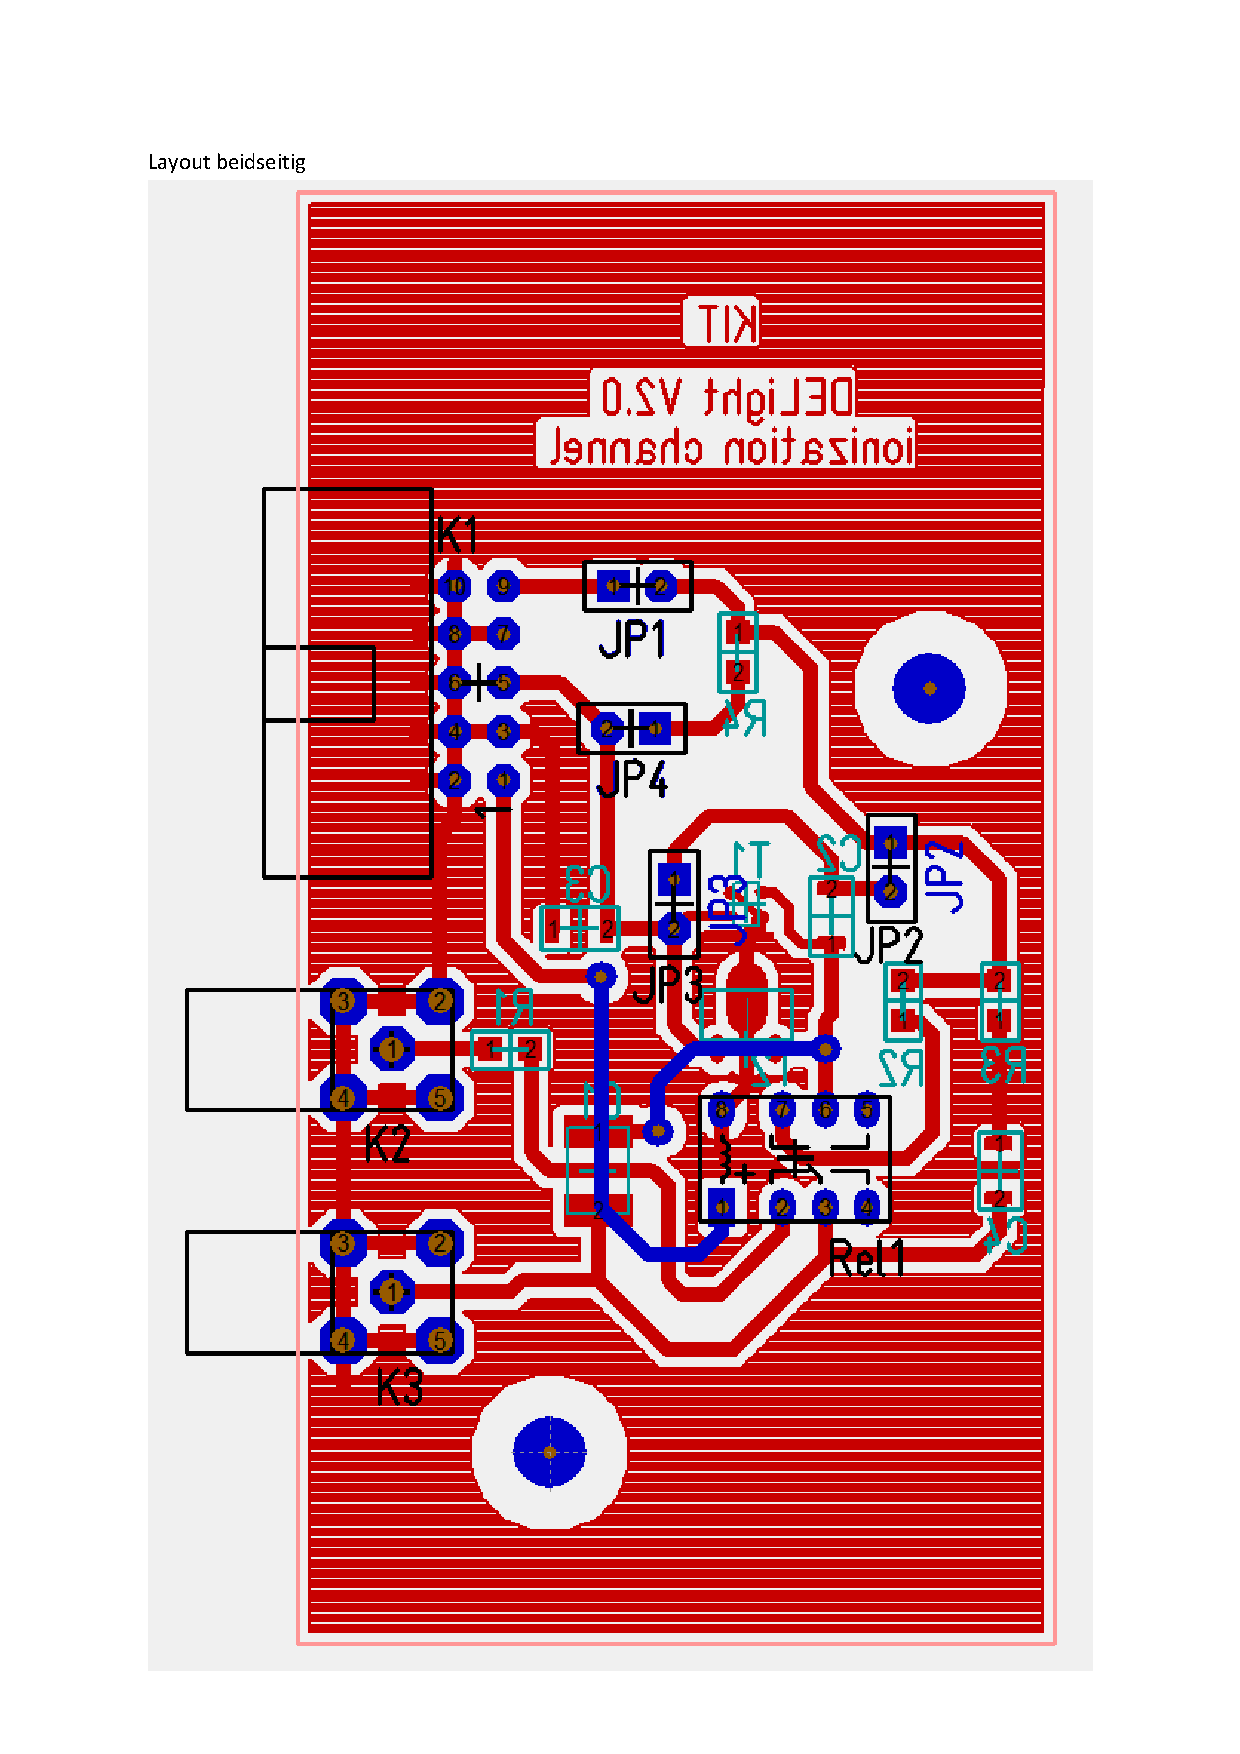
\includegraphics[page=1,width=\textwidth]{./fig/SchaltplanLayoutV2.pdf}
\vspace{-0.5cm}
\caption{Layout der kalten Elektronik}
\label{fig:Layout}
\end{center}
\end{figure}
\begin{figure}[!b]
\begin{center}
\includegraphics[page=6,width=\textwidth]{./fig/SchaltplanLayoutV2.pdf}
\vspace{-0.5cm}
\caption{Schaltplan der kalten Elektronik}
\label{fig:Schaltplan}
\end{center}
\end{figure}
    % THEBIBLIOGRAPHY
    %\begin{thebibliography}{000}
    %    \bibitem{ident}Entry into Bibliography.
    %\end{thebibliography}
\end{document}
